
This chapter presents the final, fully corrected results of the analysis described in the previous chapters. Fully corrected distributions are present, then the corrected data is compared to different MC generators using a \chisq\ test. Finally, the results of this \chisq\ test are discussed.
\section{Fully corrected distributions}
Figure~\ref{fig:unfpt} shows the normalized differential cross-section \sigmapti\ for jets of rank 1-4 and compares the data to 
four next-to-leading order generators.  Figure~\ref{fig:unfmult} provide the multiplicity of extra jets measured.
All of the generators provide a reasonable description of the leading jet. 
Correct modeling of the leading jet is perhaps unsurprising since NLO calculations can include one additional jet in the hard scattering calculation. 
Differences among the generators become larger with increasing jet rank since the generators predict significantly different rates of additional jet production. 
The generators also predict some differences in the shapes of the jet \pt\ spectra.
The \mcnlohw\ generator predicts the lowest rate of additional jet production and underestimates the number of events with at least 4 jets by ~40\%.
The level of agreement between the remaining generators and the data can only be assessed using a more rigorous statistical test and is discussed below.


The same fully corrected data are compared to multi-leg leading order generators in Figure~\ref{fig:unfptmllo}.  In all cases, the renormalization and
factorization scales are set to the defaults provided by the code authors.  Alpgen used with \py\ or \hw\ does a reasonable job of reproducing the data, while \madpy\ provides a less accurate description.

 For lowest order generators, the predicted cross section can depend strongly on the choice of 
scale.  Figure~\ref{fig:unfptlosys} shows the effects of such scale variation for the generators under consideration.  In all cases the solid
(dashed) line shows the predicted rate with the scale is halved (doubled).  The measurement provides a smaller uncertainty on the cross section than the 
scale variations in the lowest order calculation would allow.
\begin{figure}
\centering
\subfloat{
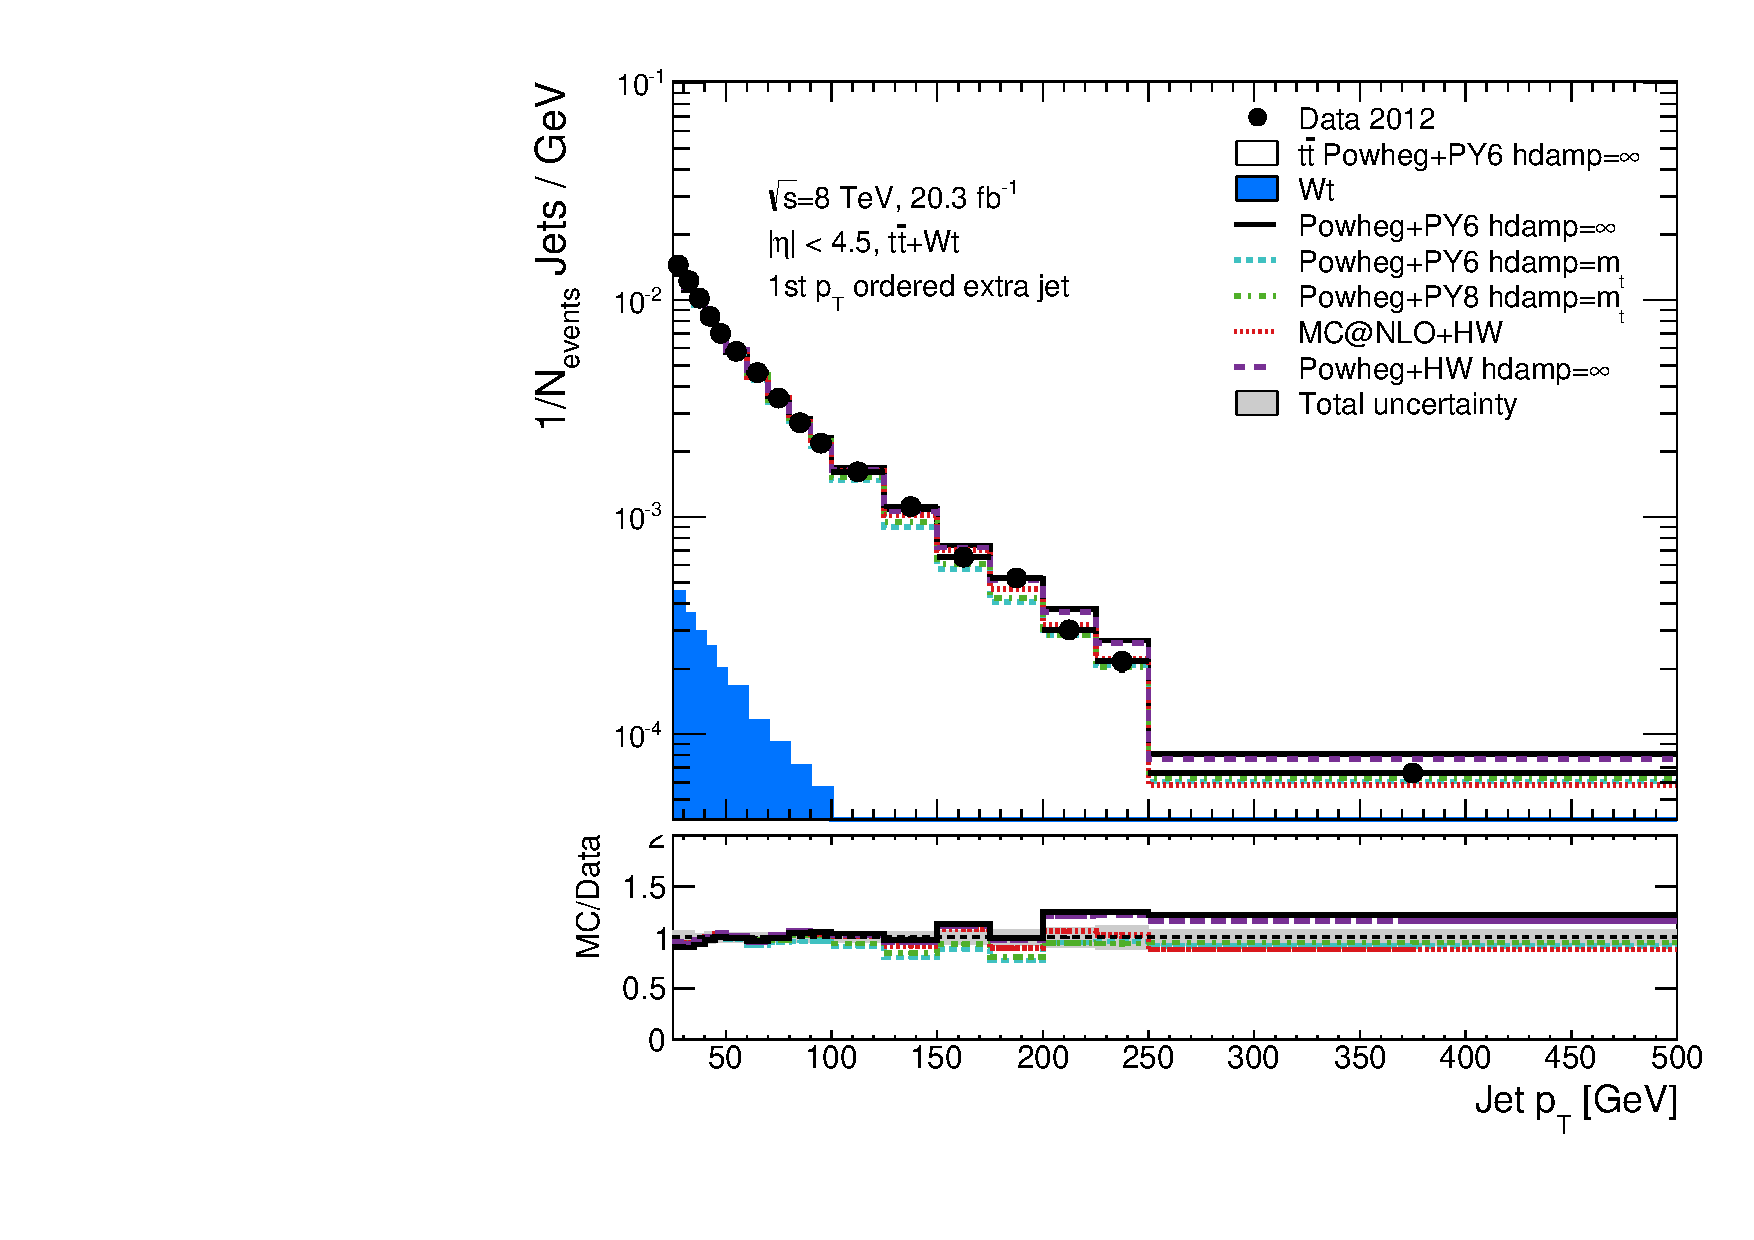
\includegraphics[width=0.45\textwidth]{fig/DataUnfold/NLO/PtJet0.pdf}}
\subfloat{
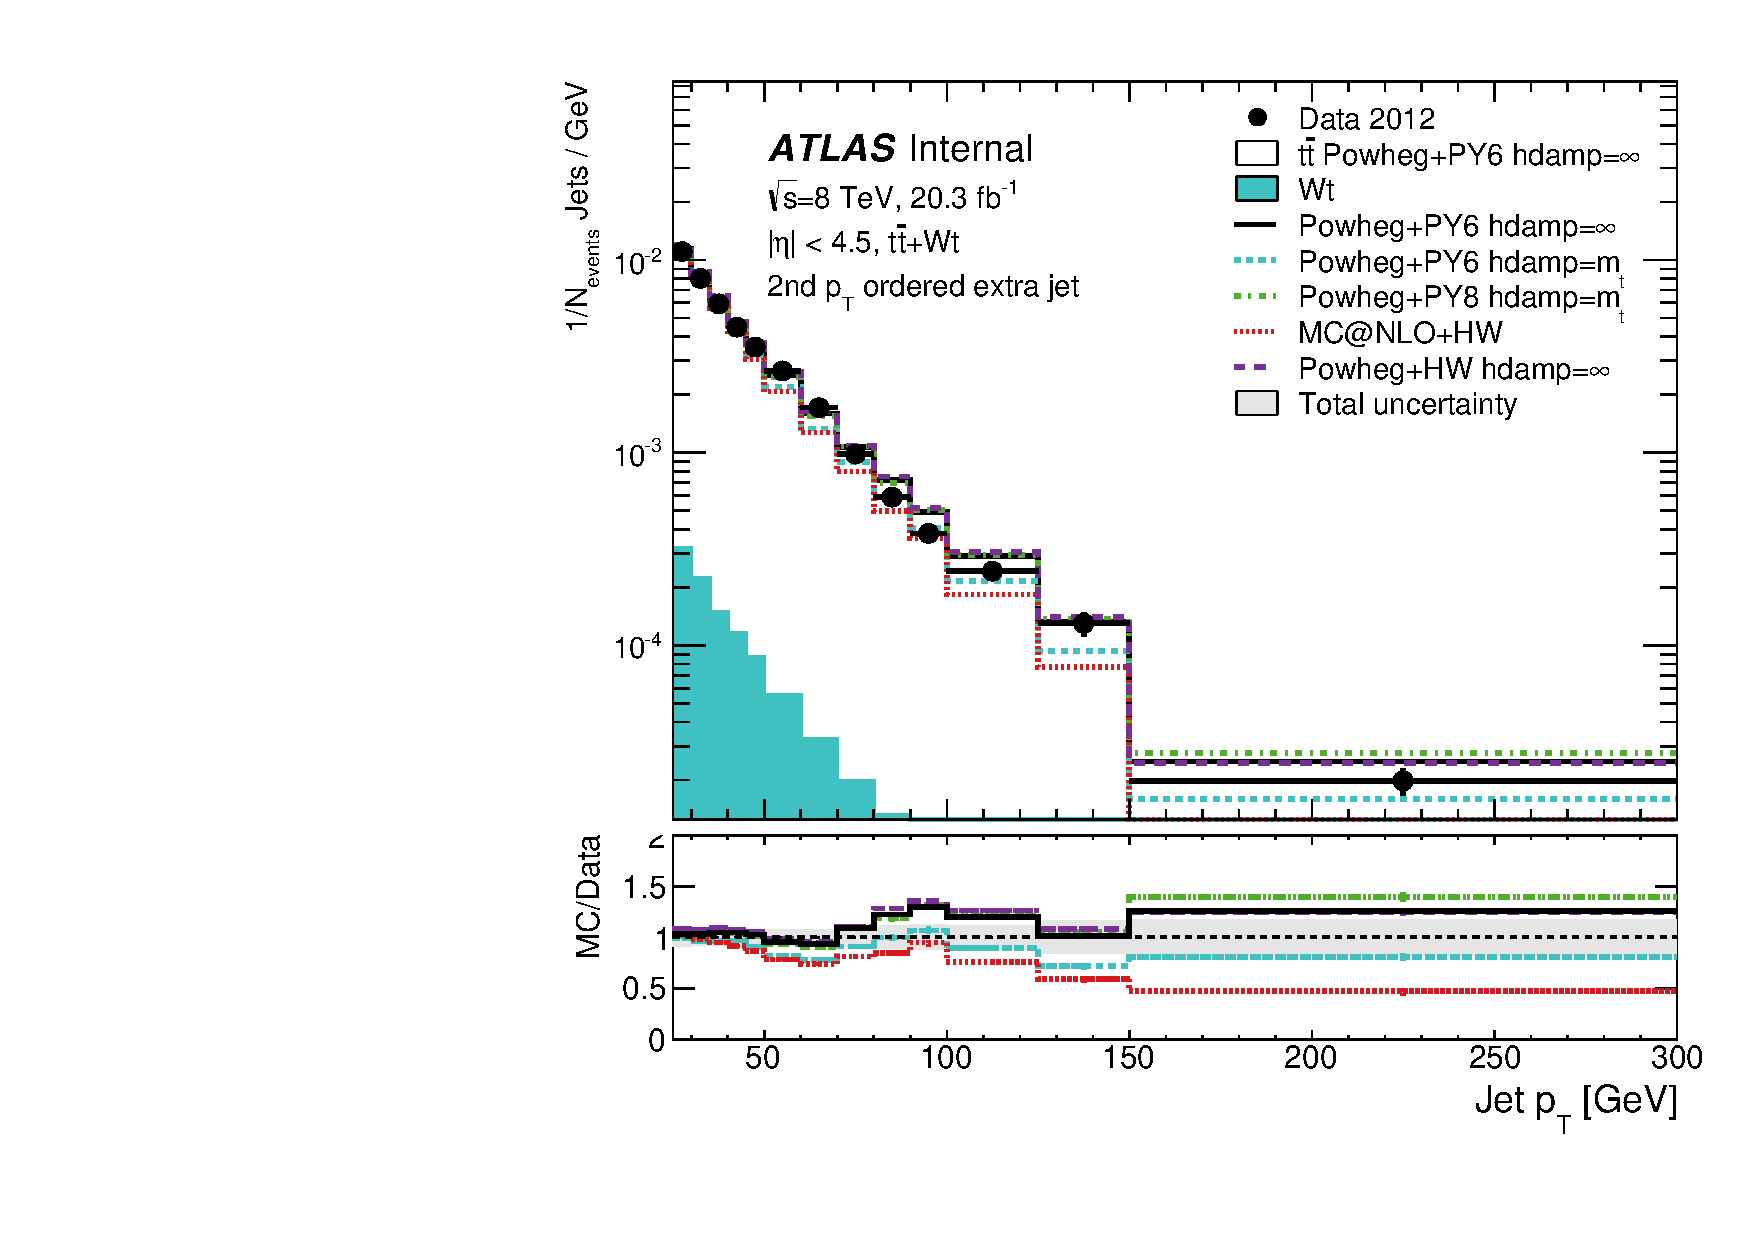
\includegraphics[width=0.45\textwidth]{fig/DataUnfold/NLO/PtJet1.pdf}} \\
\subfloat{
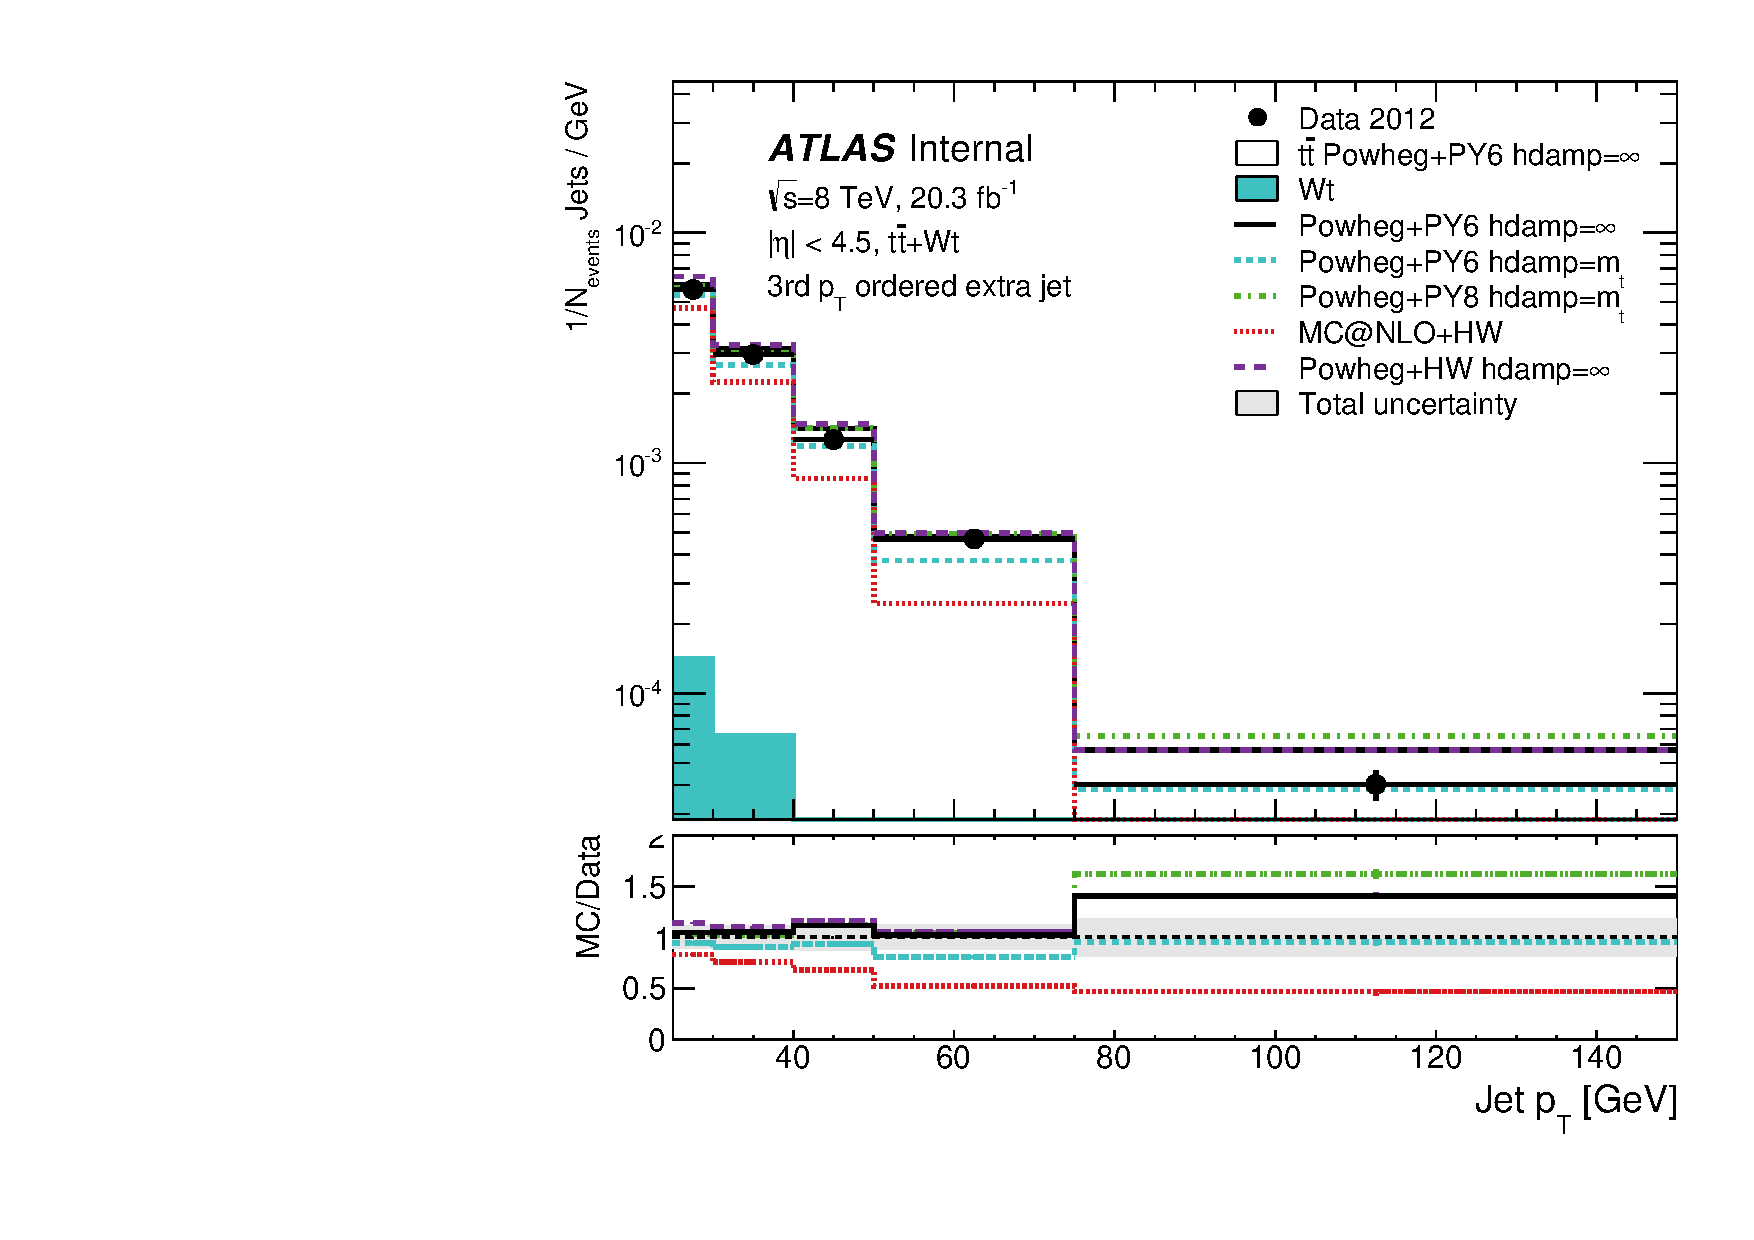
\includegraphics[width=0.45\textwidth]{fig/DataUnfold/NLO/PtJet2.pdf}}
\subfloat{
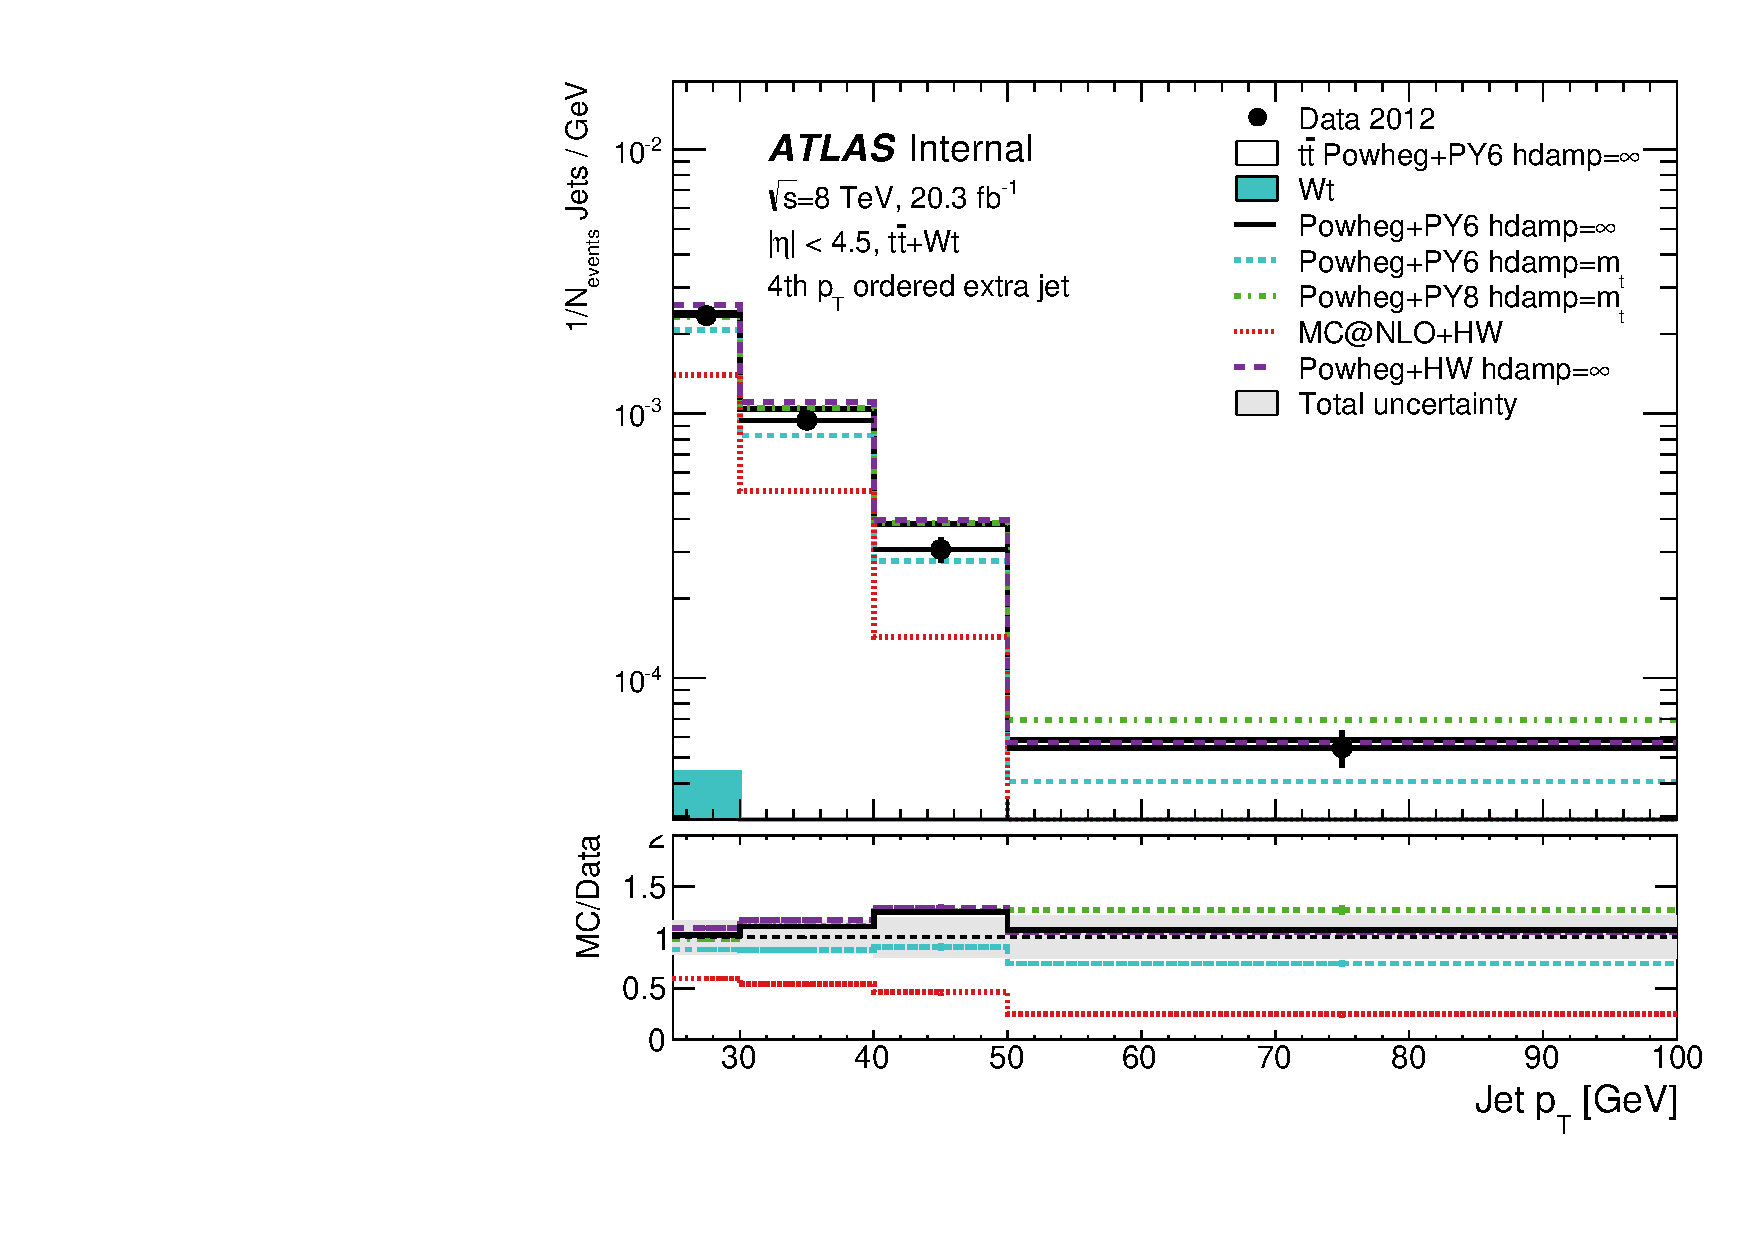
\includegraphics[width=0.45\textwidth]{fig/DataUnfold/NLO/PtJet3.pdf}} 
% \subfloat{
% 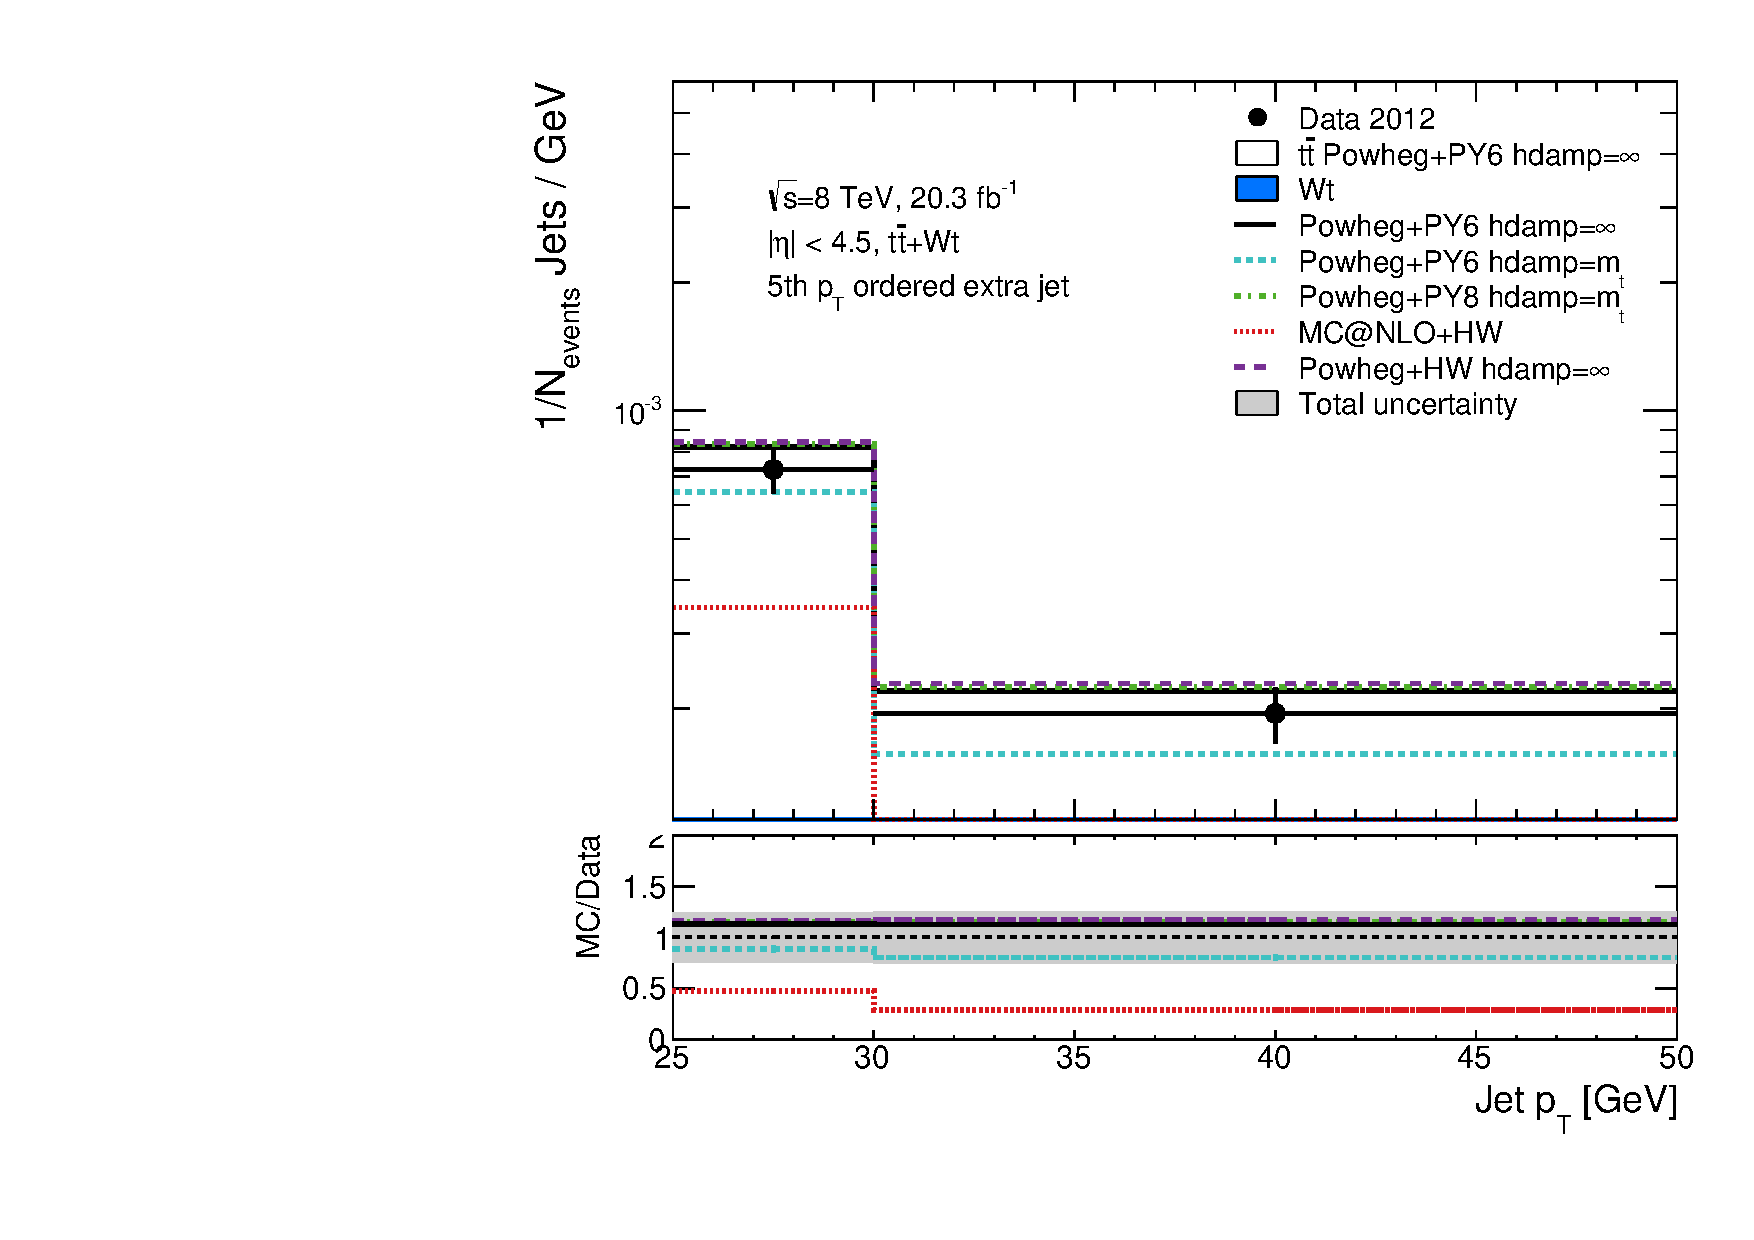
\includegraphics[width=0.45\textwidth]{fig/DataUnfold/NLO/PtJet4.pdf}}
\caption{Distributions of the unfolded \pt of extra jets in data and simulation. Each sample is unfolded against a response matrix filled with baseline \ttbar+single top simulation. The gray band on the ratio shows the sum of statistical and systematic uncertainties.}
\label{fig:unfpt}
\end{figure}

\begin{figure}
\centering
\subfloat{
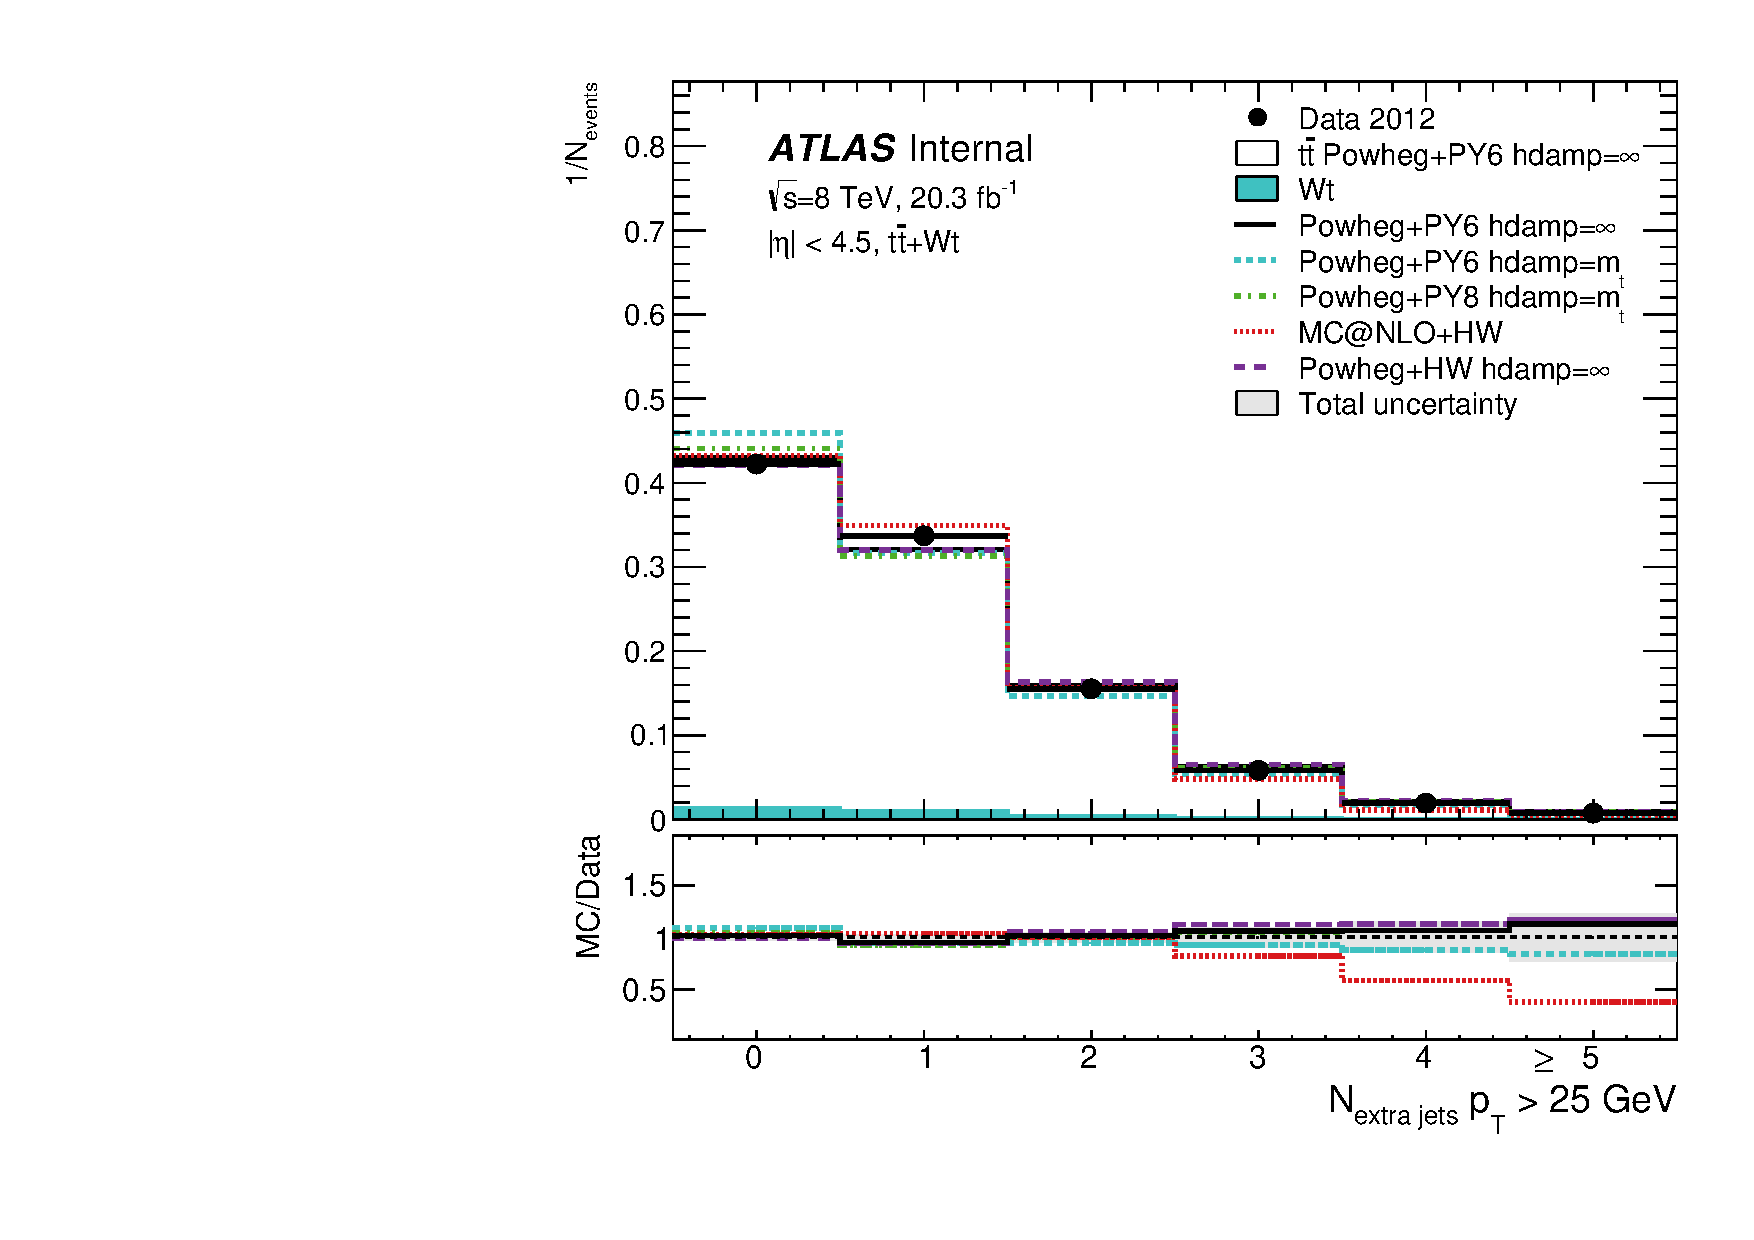
\includegraphics[width=0.45\textwidth]{fig/DataUnfold/NLO/NExtraJets25.pdf}}
\subfloat{
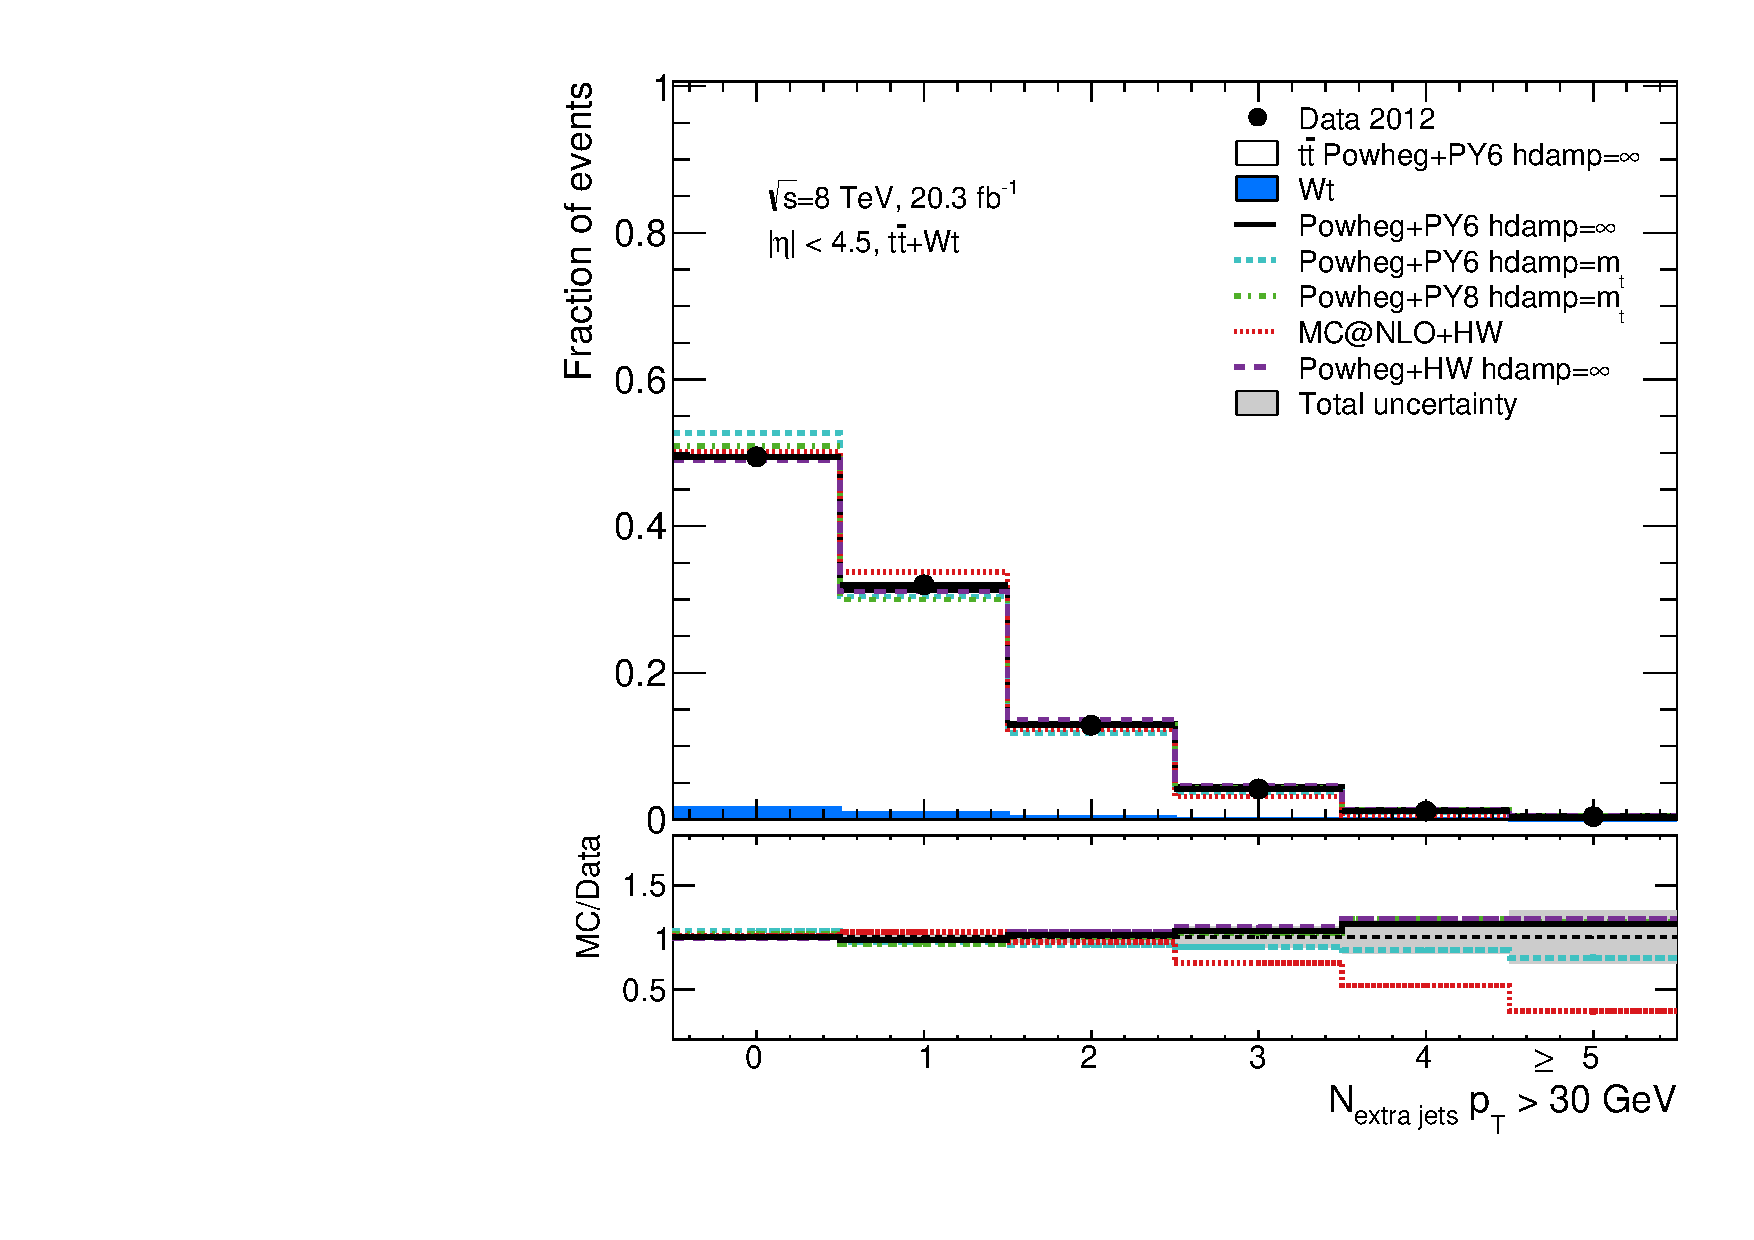
\includegraphics[width=0.45\textwidth]{fig/DataUnfold/NLO/NExtraJets30.pdf}}
\\
\subfloat{
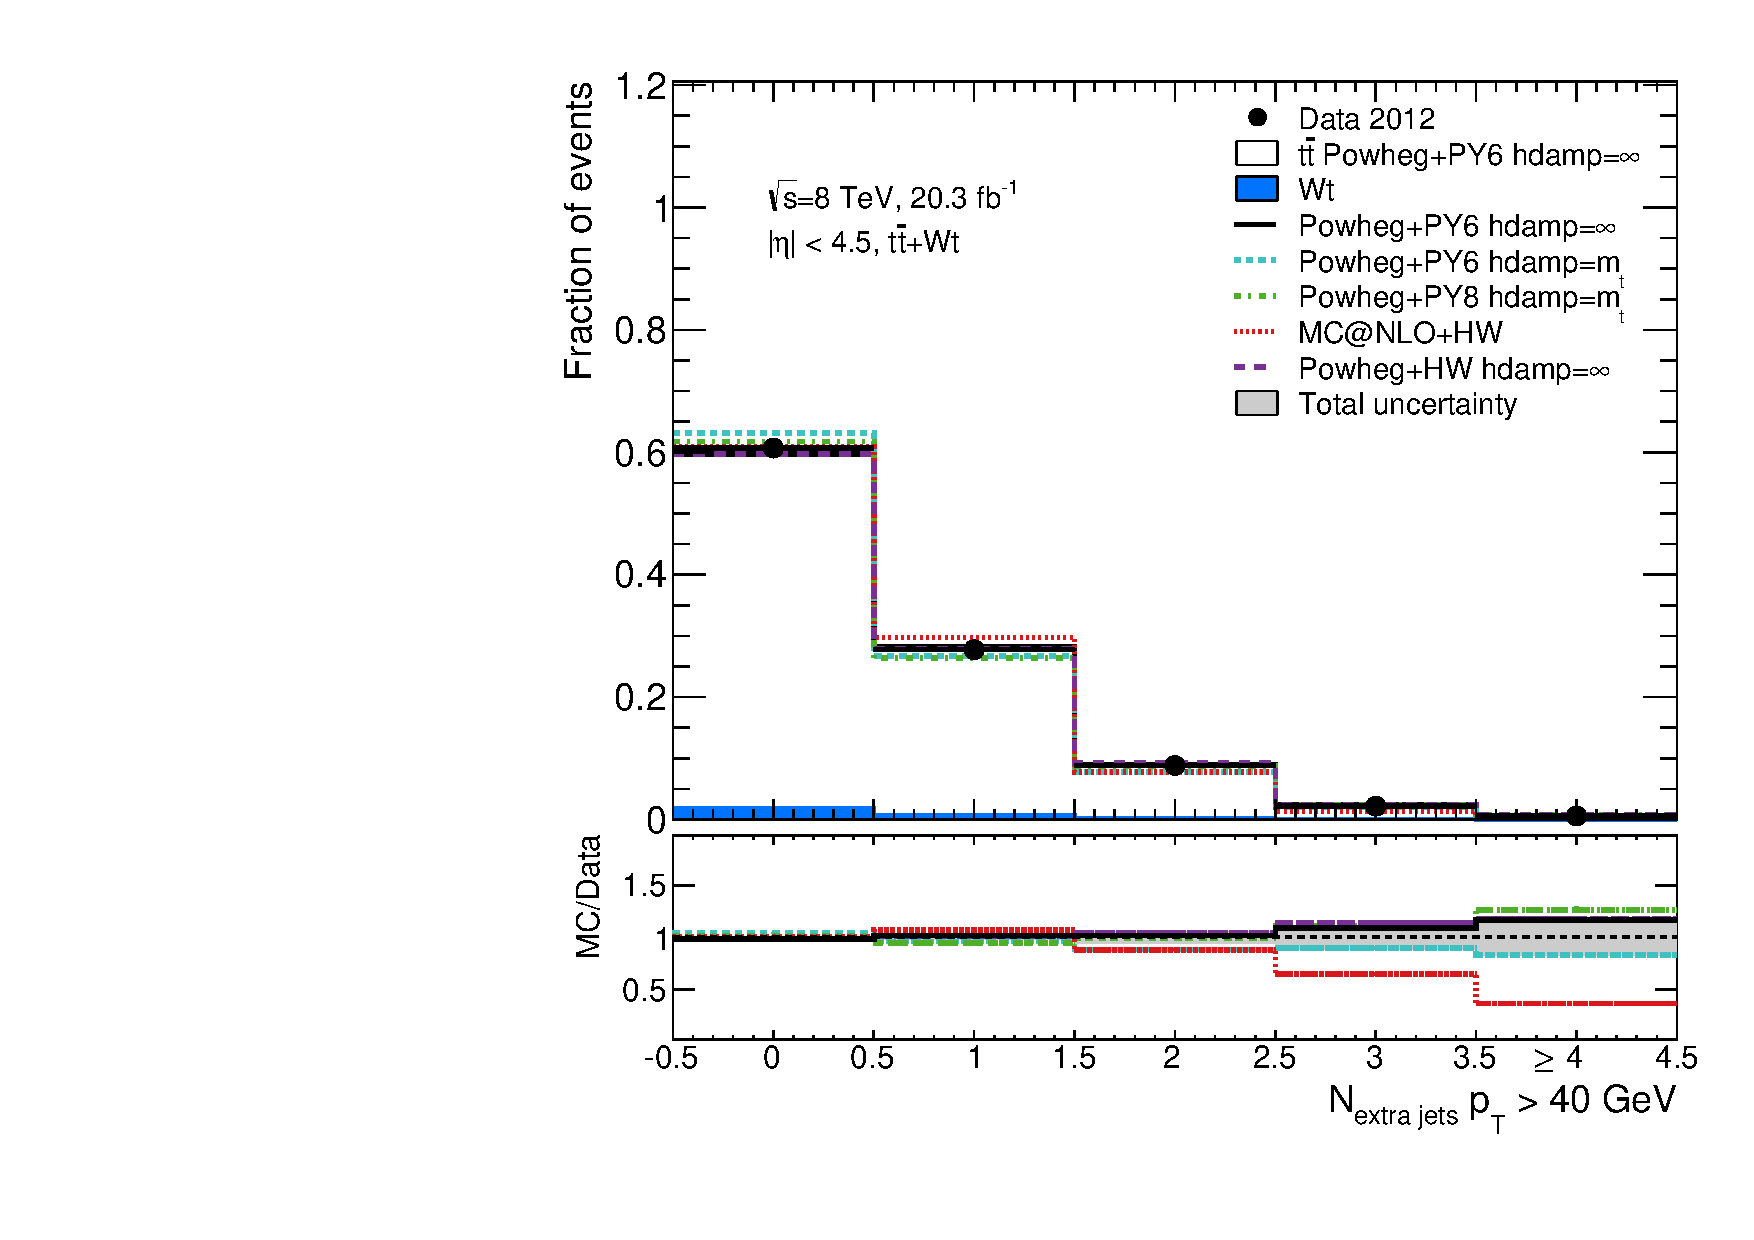
\includegraphics[width=0.45\textwidth]{fig/DataUnfold/NLO/NExtraJets40.pdf}}
\subfloat{
%\includegraphics[width=0.45\textwidth]{fig/DataUnfold/NLO/NExtraPt50.pdf}}
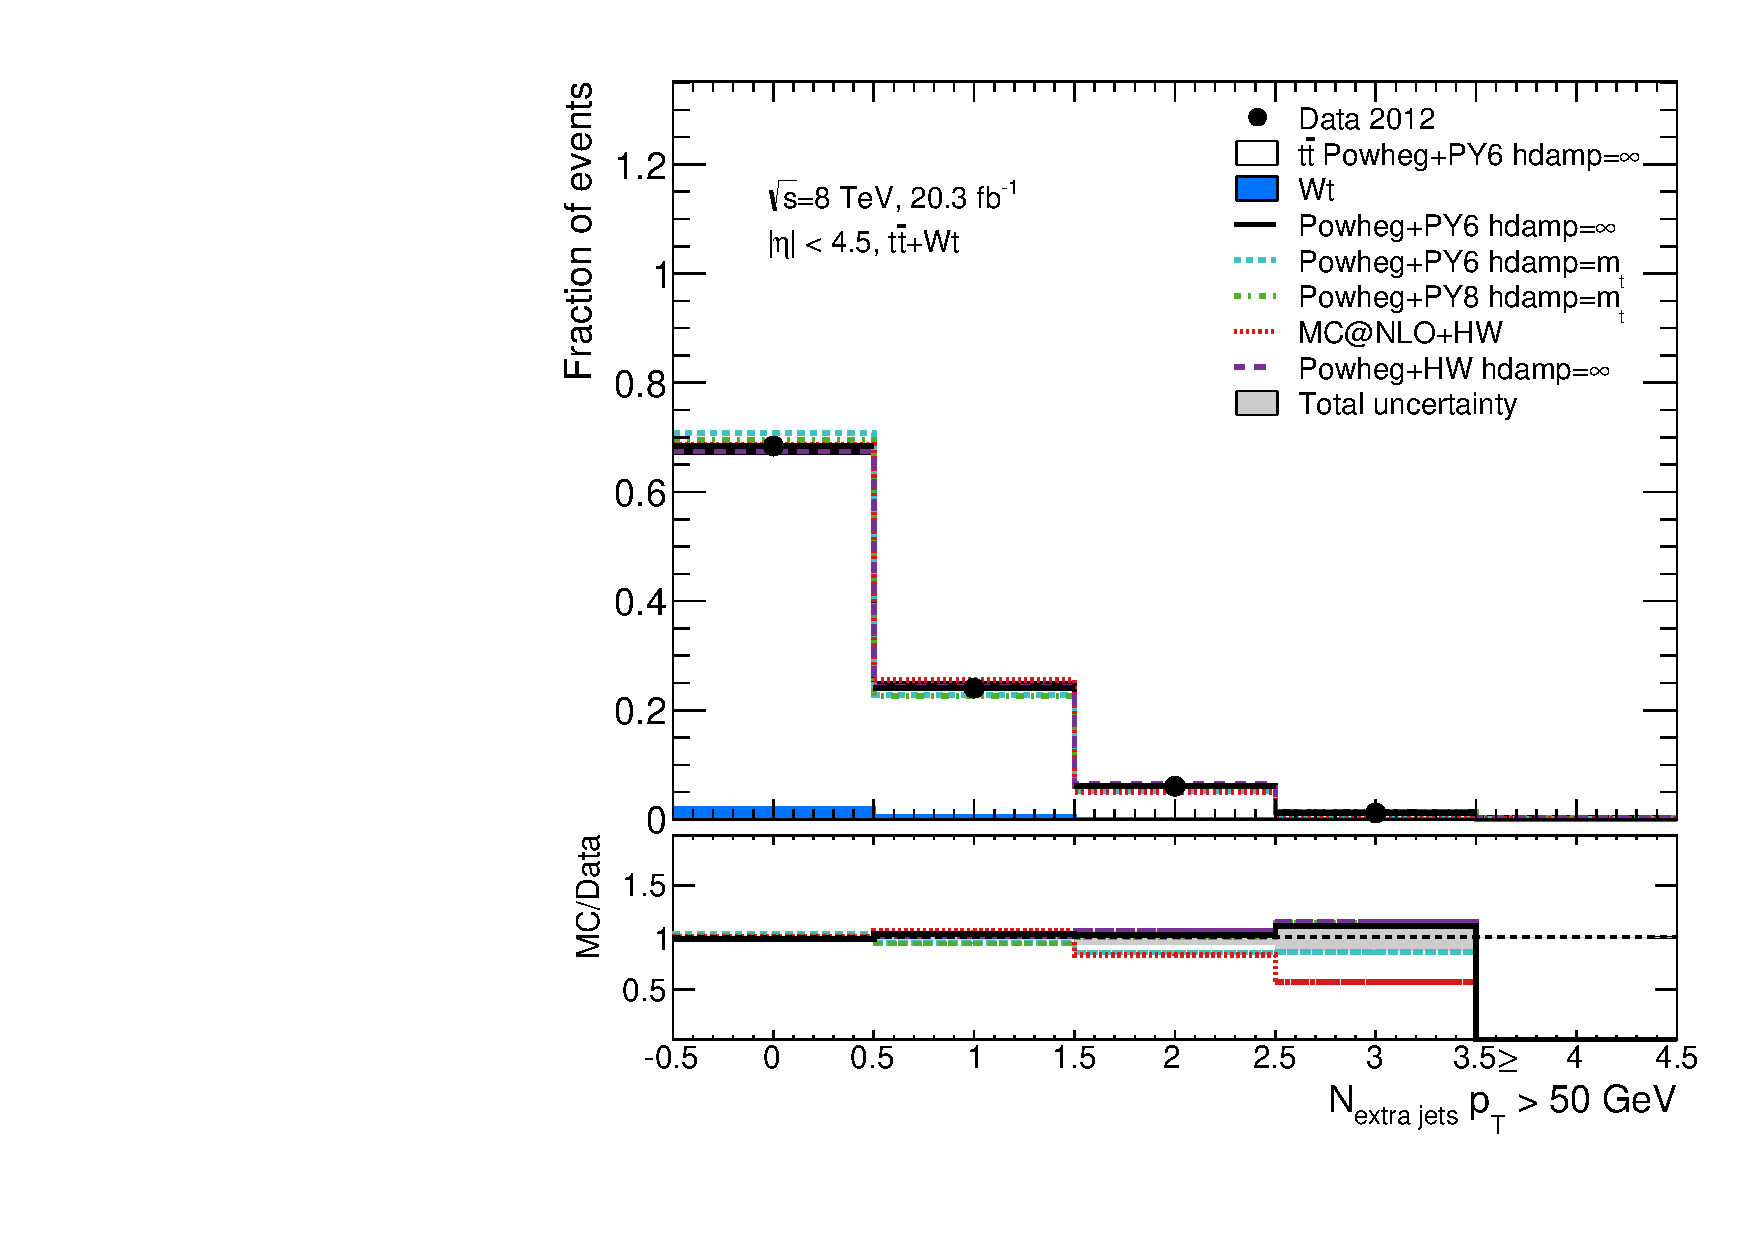
\includegraphics[width=0.45\textwidth]{fig/DataUnfold/NLO/NExtraJets50.pdf}}
\caption{Distributions of the number of unfolded extra jets with \pt > (a) 25, (b) 30, (c) 40 and (d) 50 \GeV\ in data and simulation.  Each sample is unfolded against a response matrix filled with baseline \ttbar+single top simulation. The gray band on the ratio shows the sum of statistical and systematic uncertainties.}
\label{fig:unfmult}
\end{figure}


\begin{figure}
\centering
\subfloat{
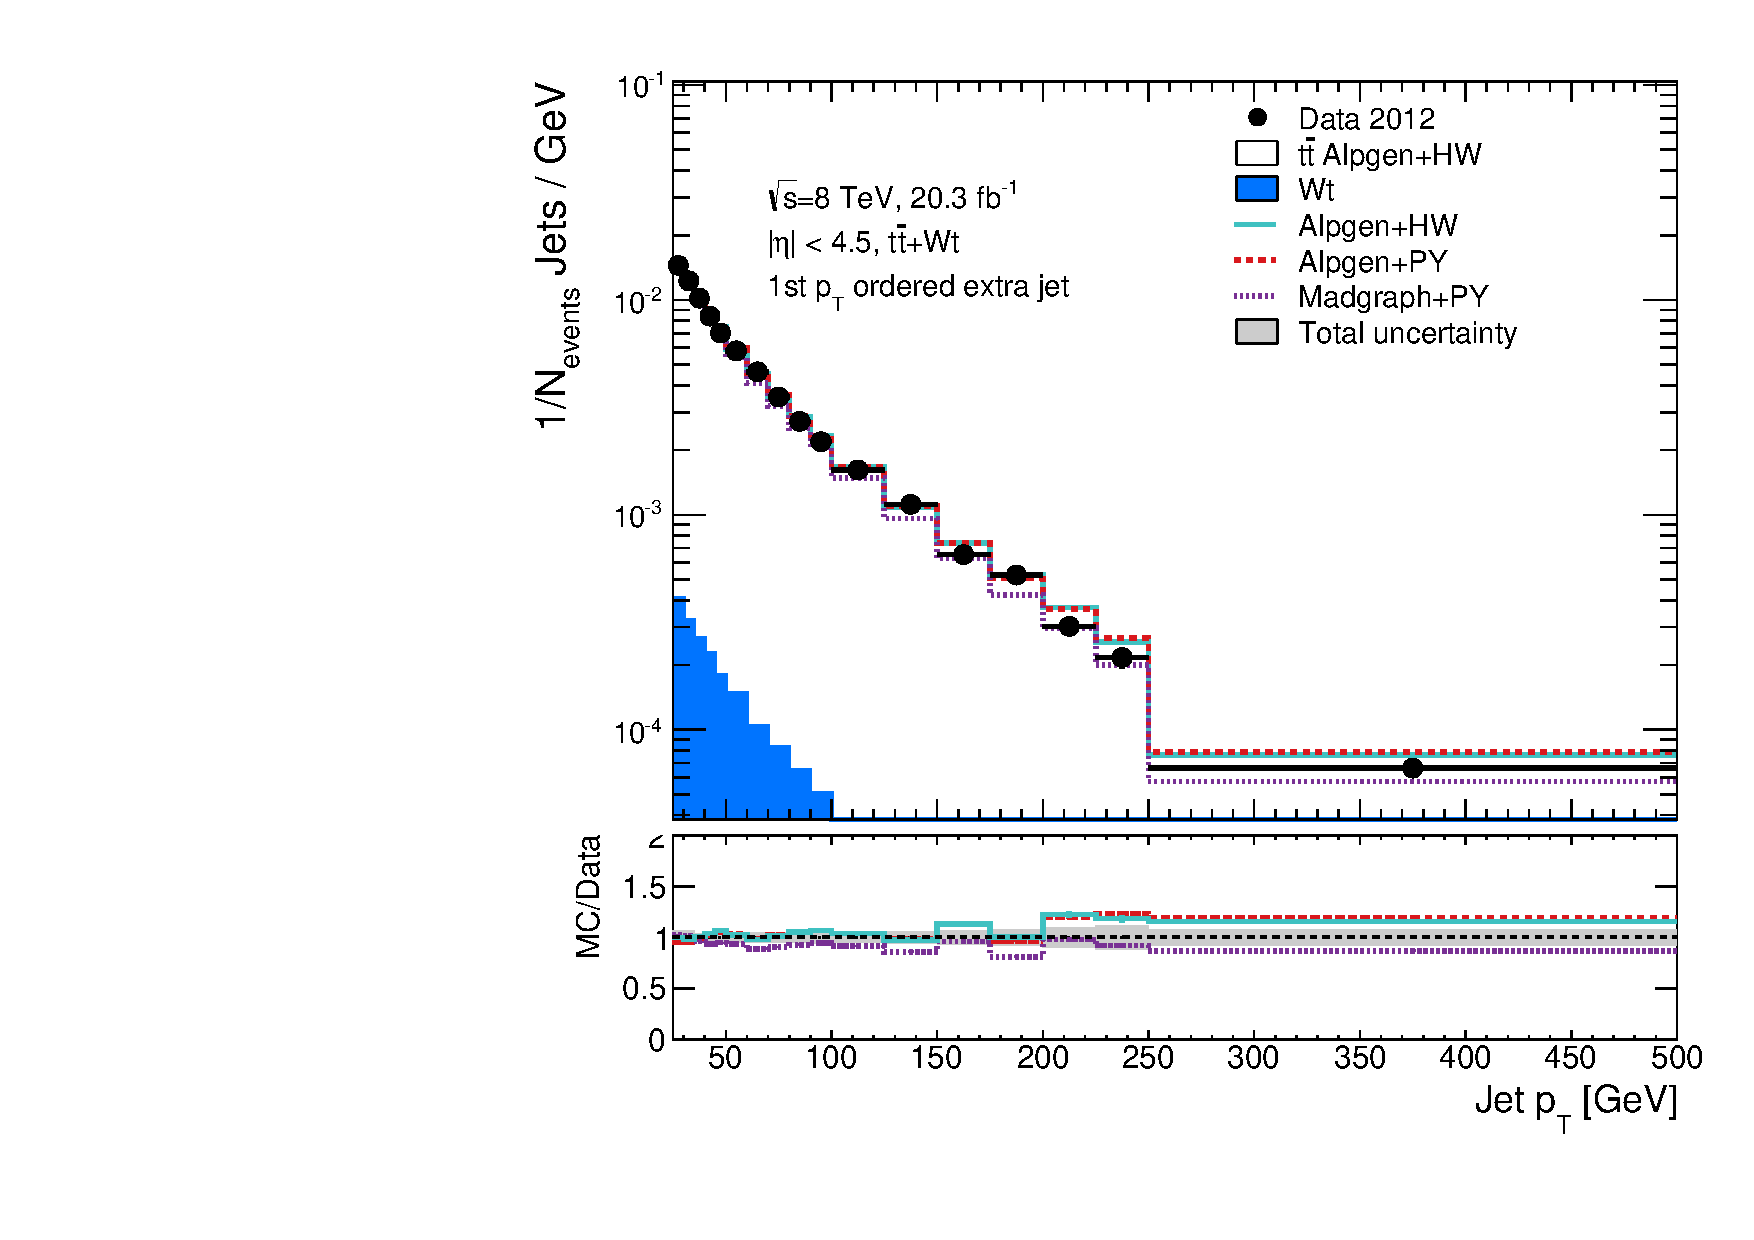
\includegraphics[width=0.45\textwidth]{fig/DataUnfold/LOMultiLeg/PtJet0.pdf}}
\subfloat{
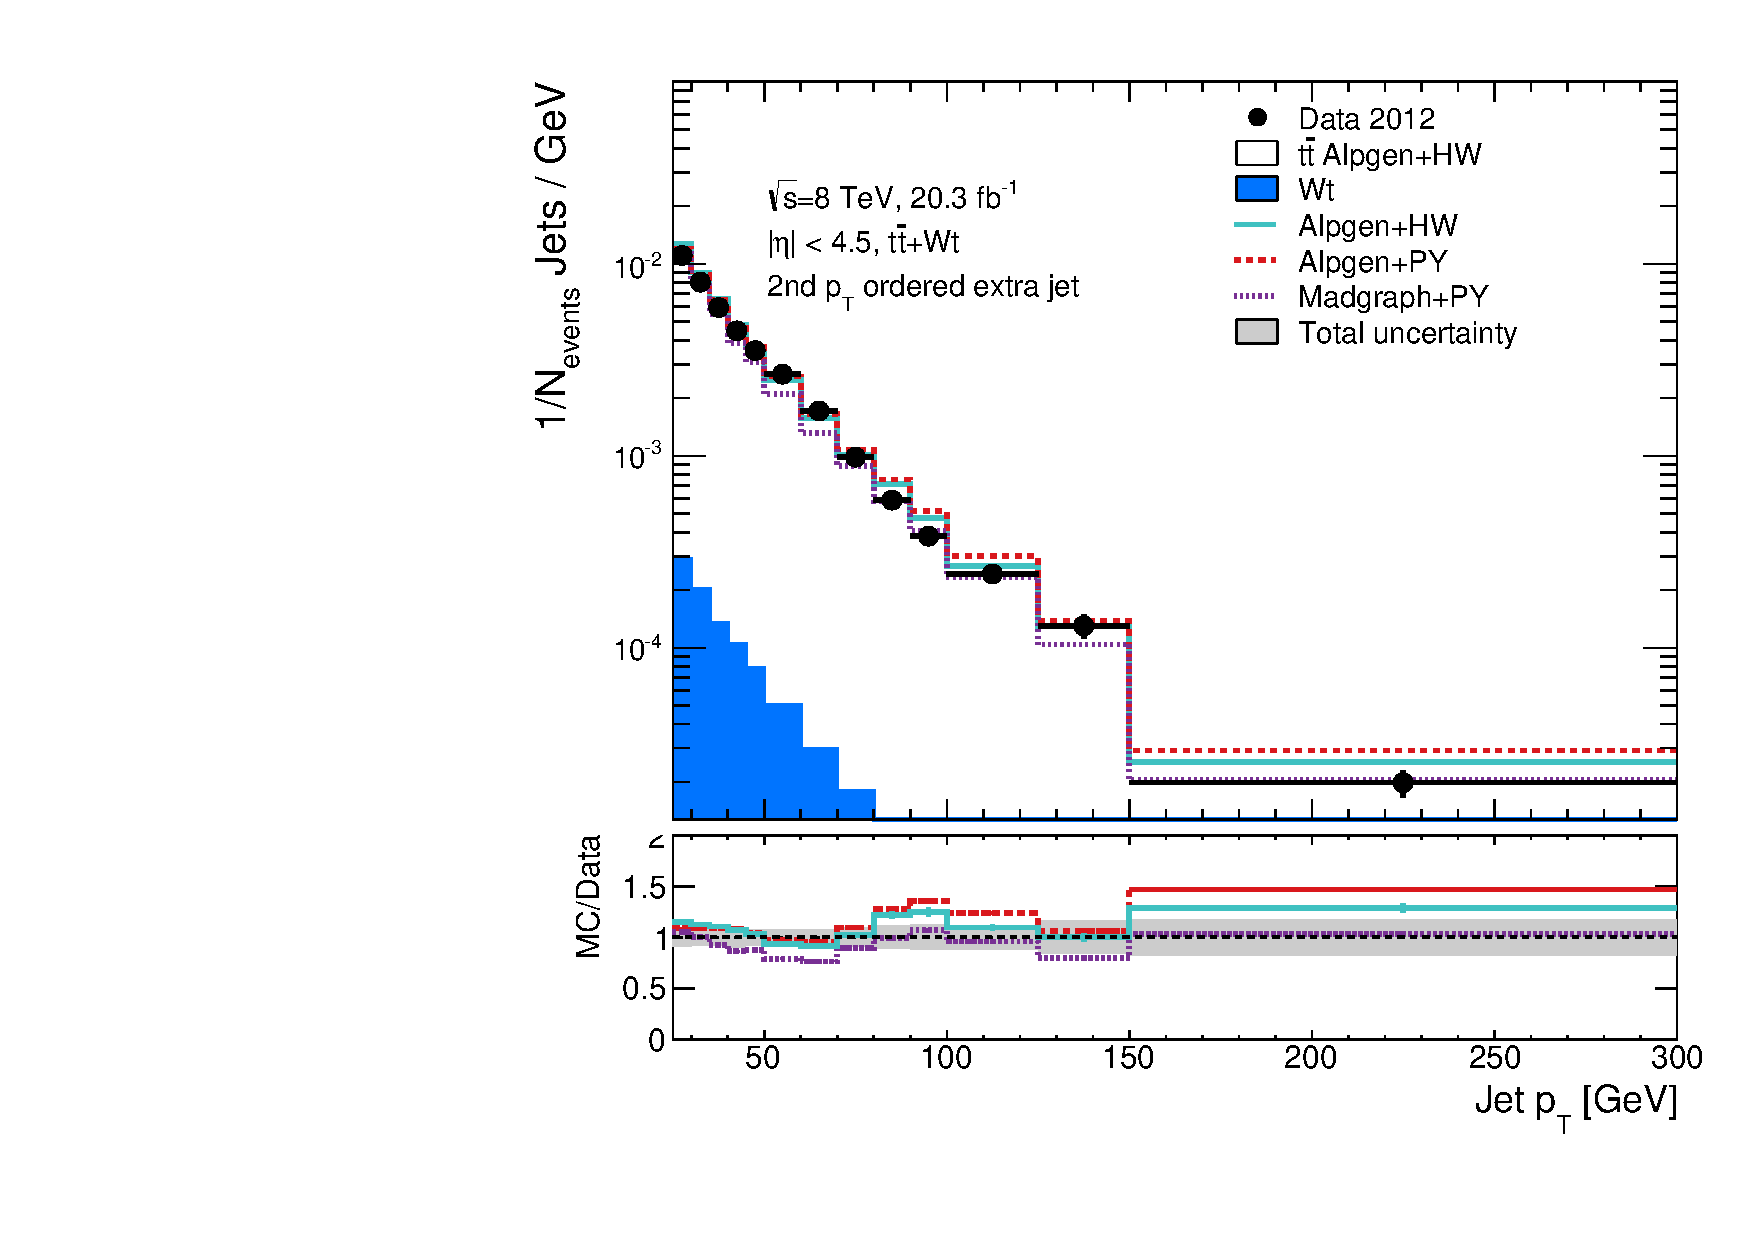
\includegraphics[width=0.45\textwidth]{fig/DataUnfold/LOMultiLeg/PtJet1.pdf}} \\
\subfloat{
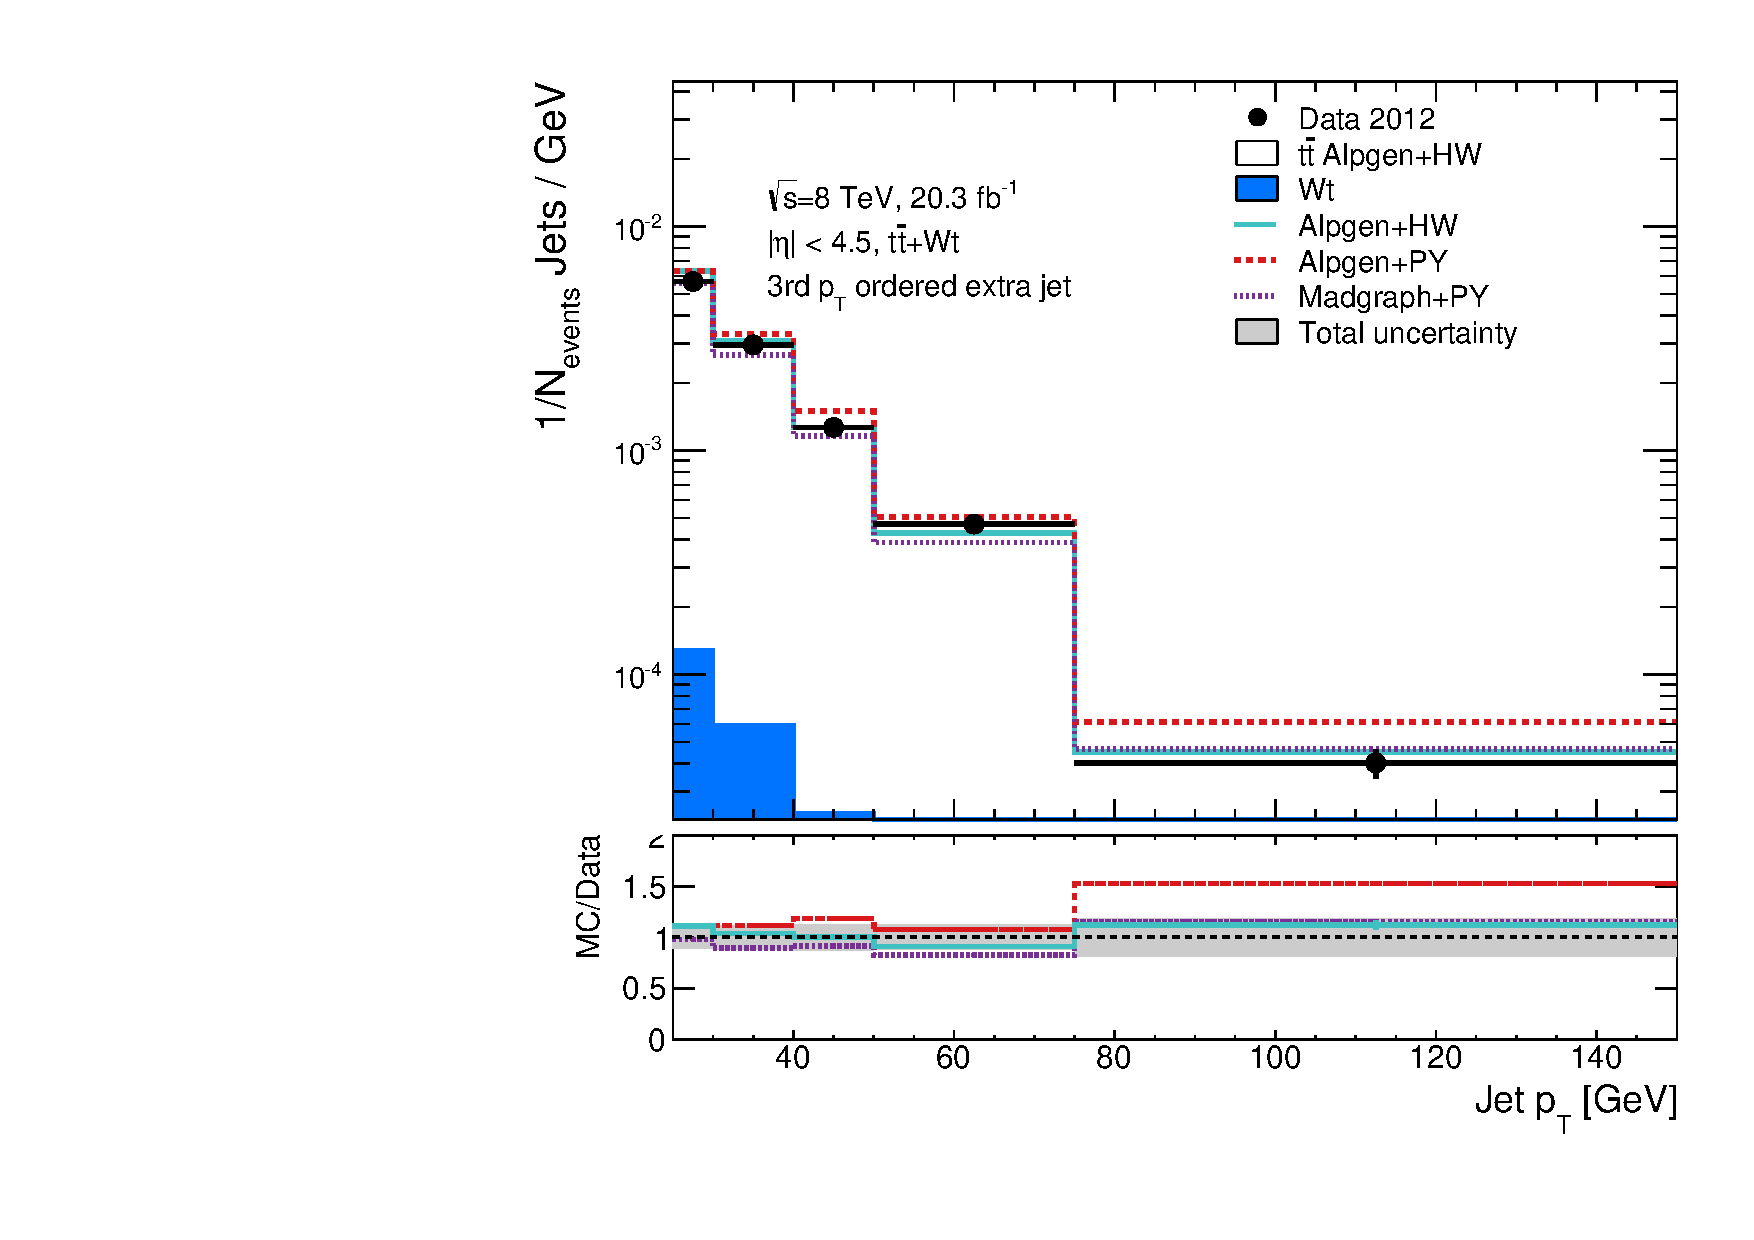
\includegraphics[width=0.45\textwidth]{fig/DataUnfold/LOMultiLeg/PtJet2.pdf}}
\subfloat{
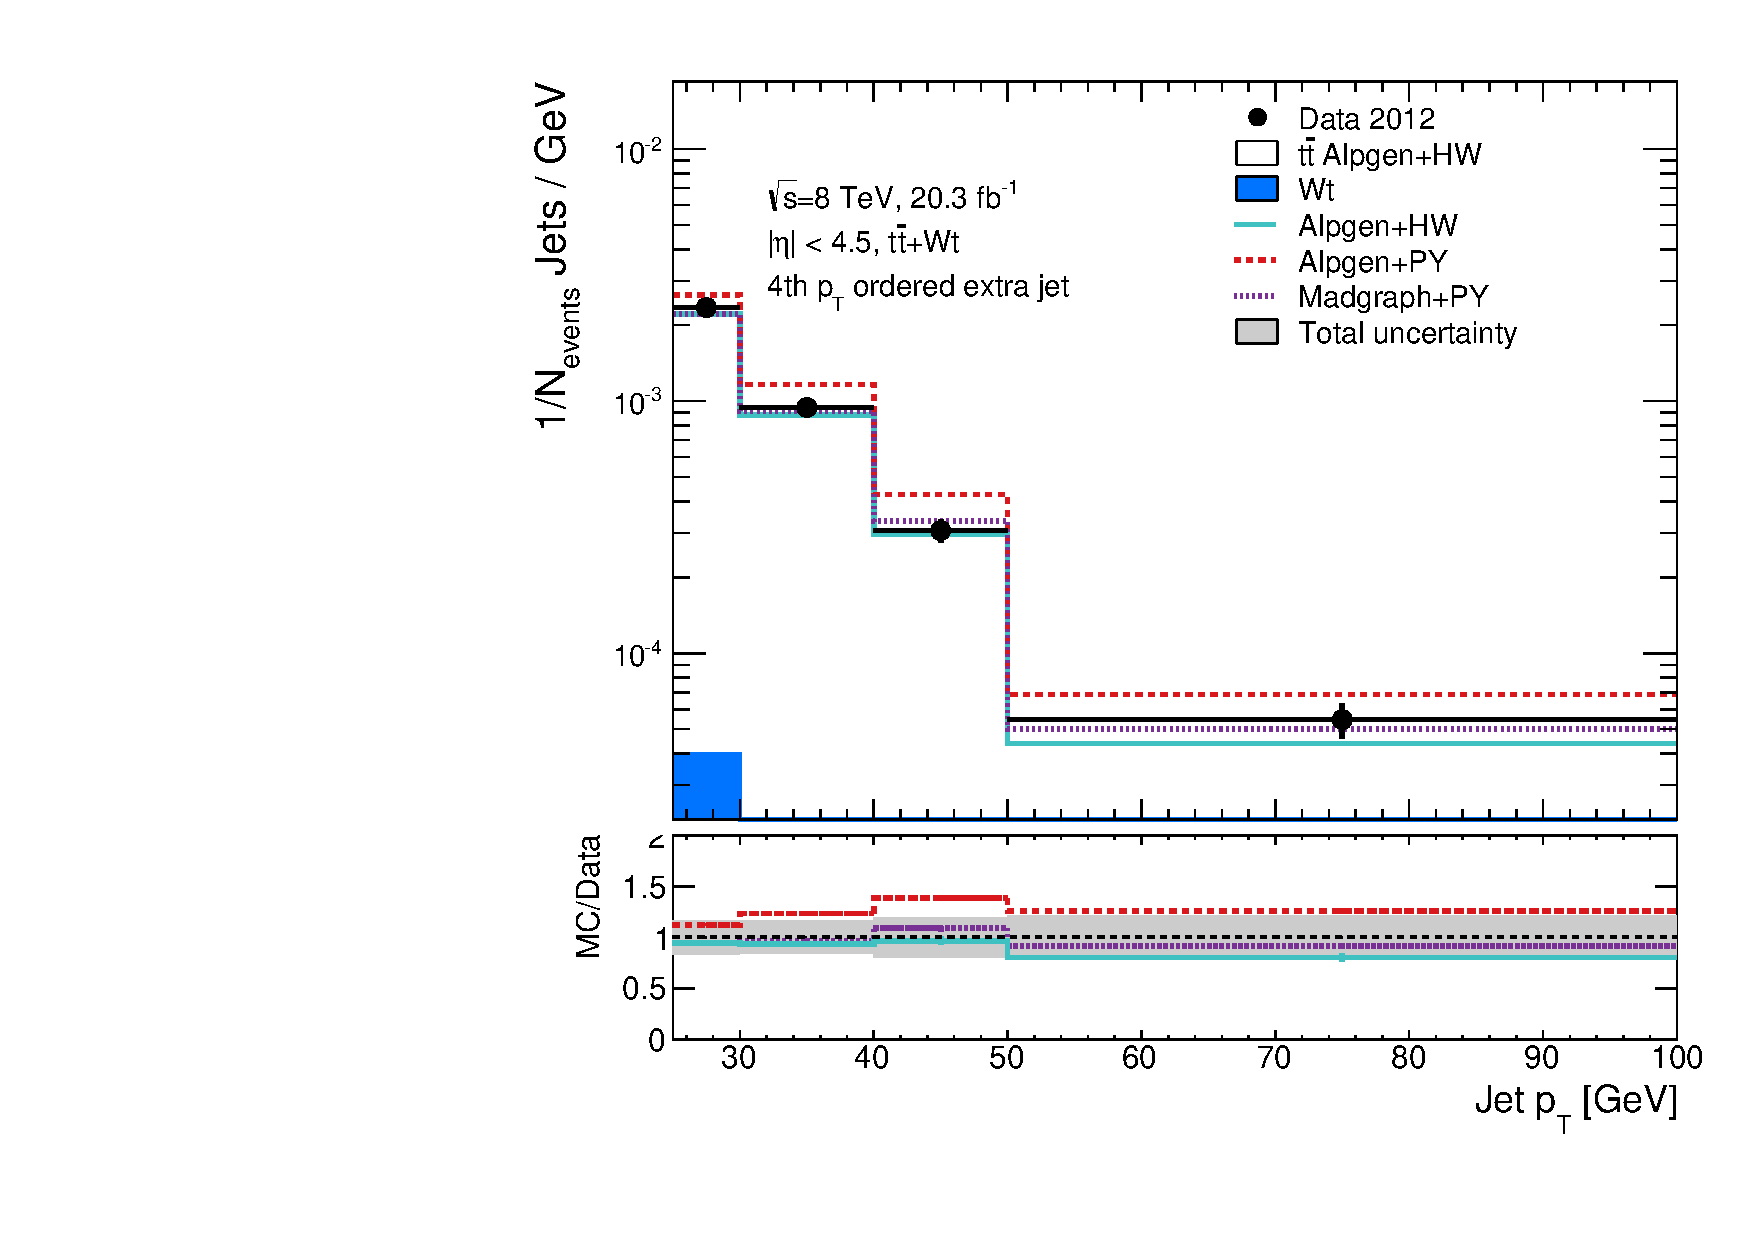
\includegraphics[width=0.45\textwidth]{fig/DataUnfold/LOMultiLeg/PtJet3.pdf}} 
\caption{Distributions of the unfolded \pt of extra jets in data and simulation. Each sample is unfolded against a response matrix filled with baseline \ttbar+single top simulation. The gray band on the ratio shows the sum of statistical and systematic uncertainties.}
\label{fig:unfptmllo}
\end{figure}
\begin{figure}
\centering
\subfloat{
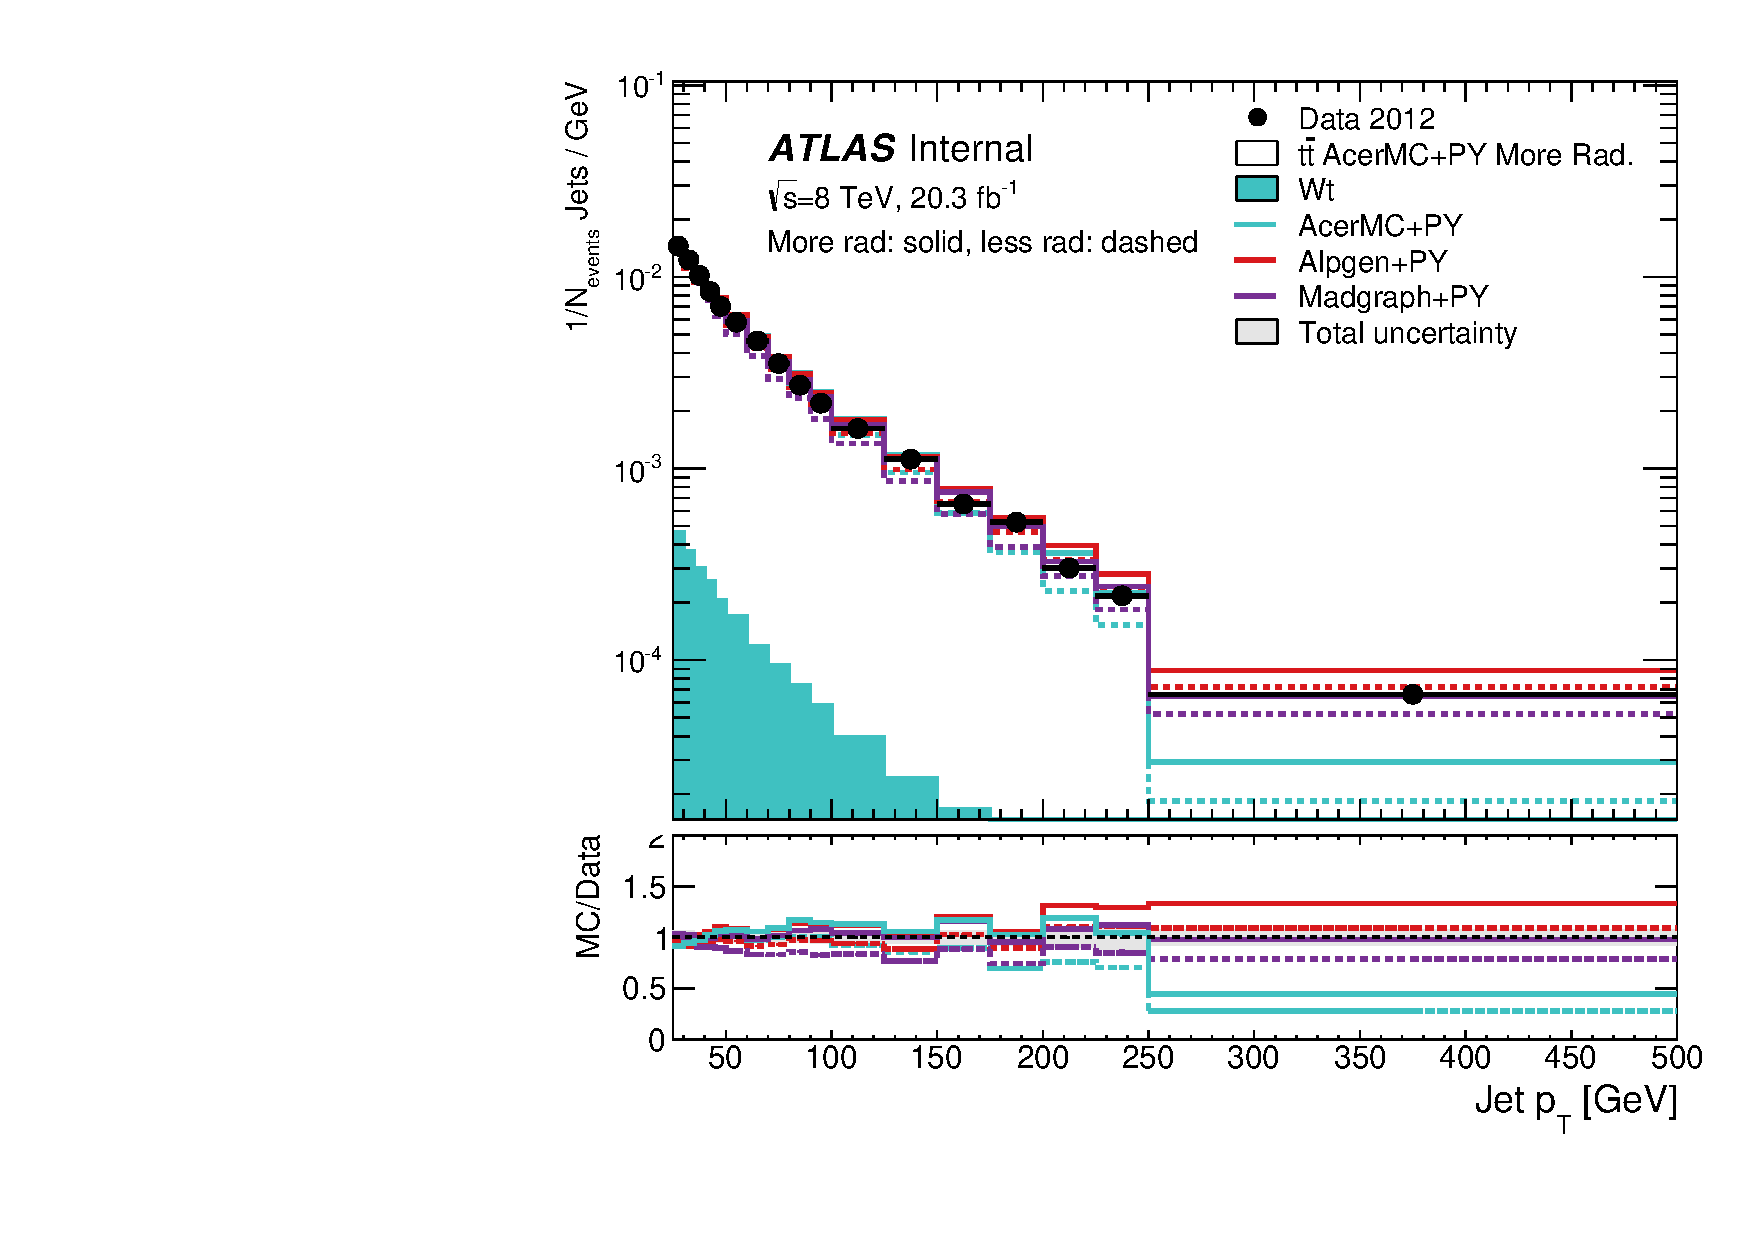
\includegraphics[width=0.45\textwidth]{fig/DataUnfold/LOSys/PtJet0.pdf}}
\subfloat{
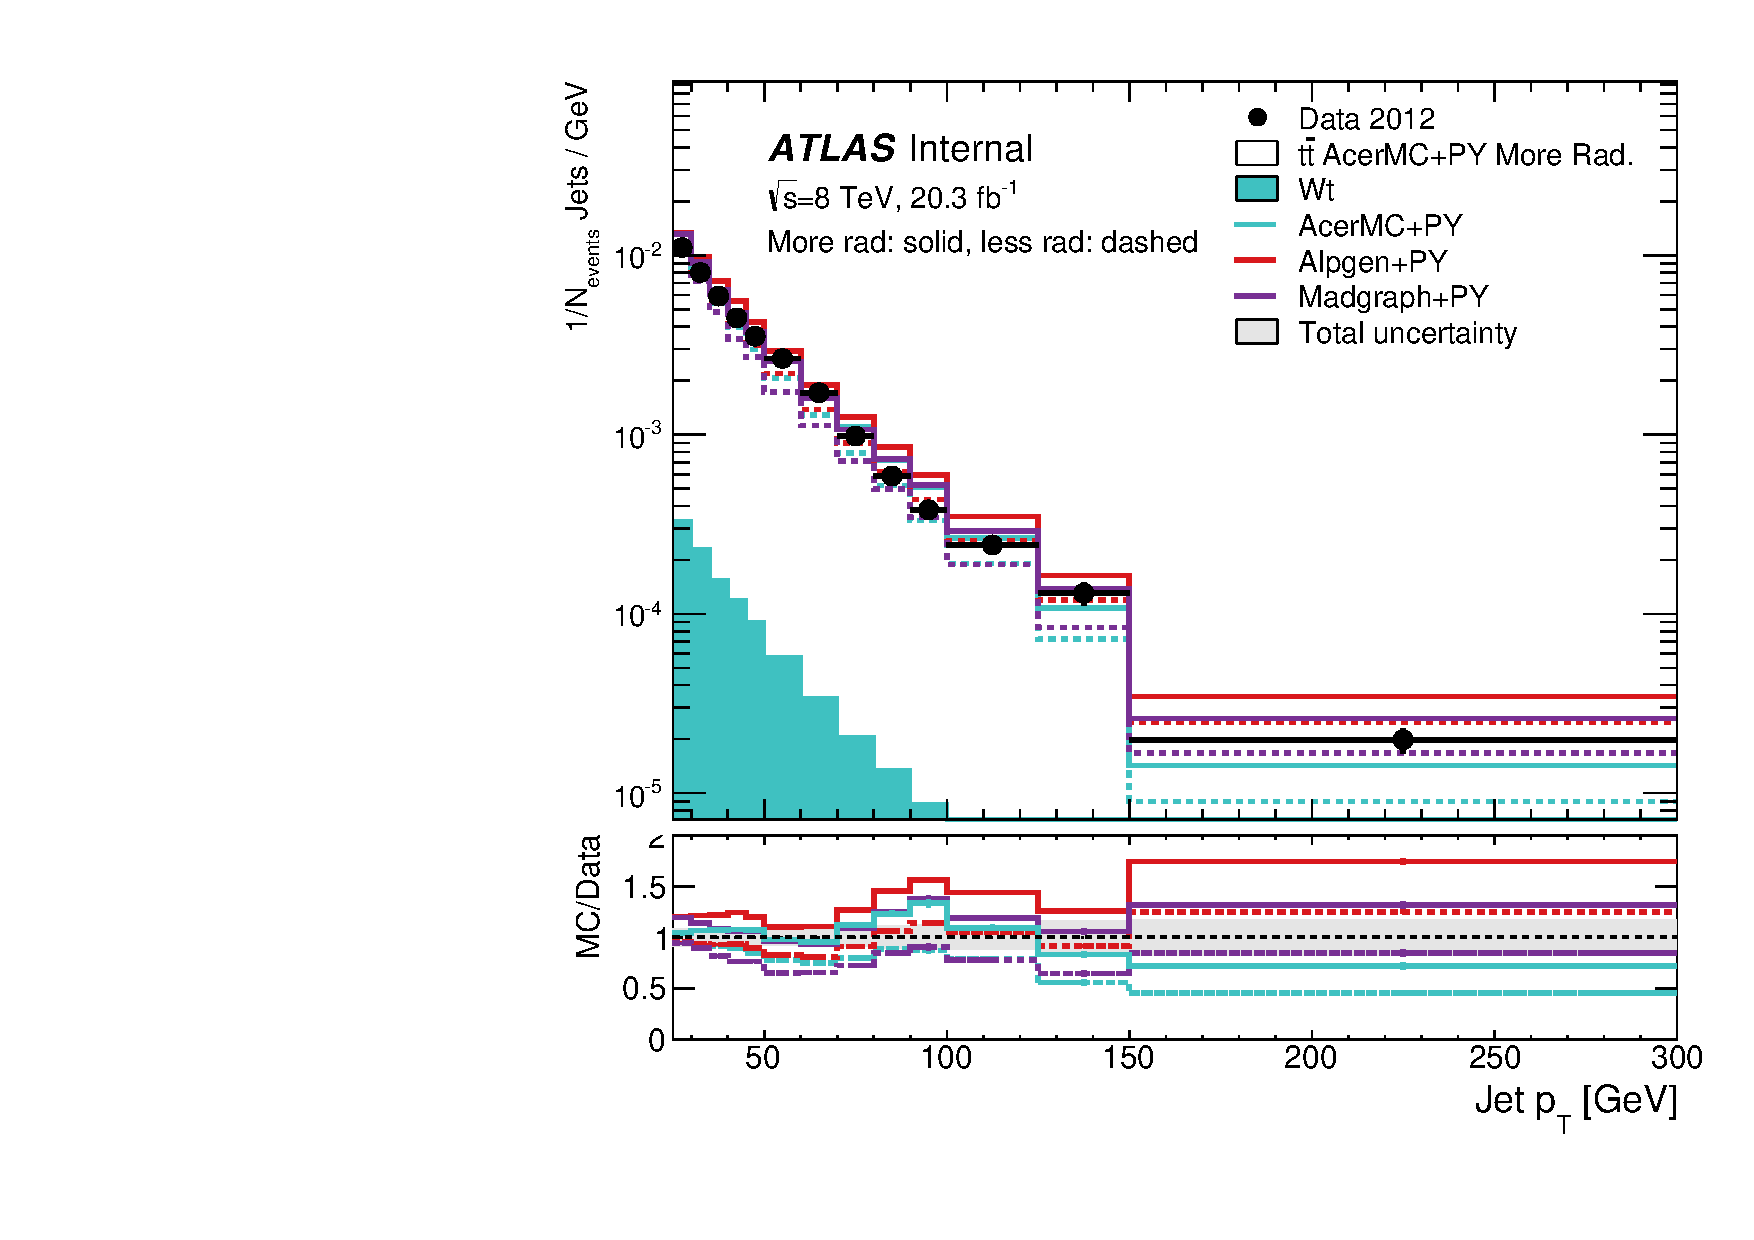
\includegraphics[width=0.45\textwidth]{fig/DataUnfold/LOSys/PtJet1.pdf}} \\
\subfloat{
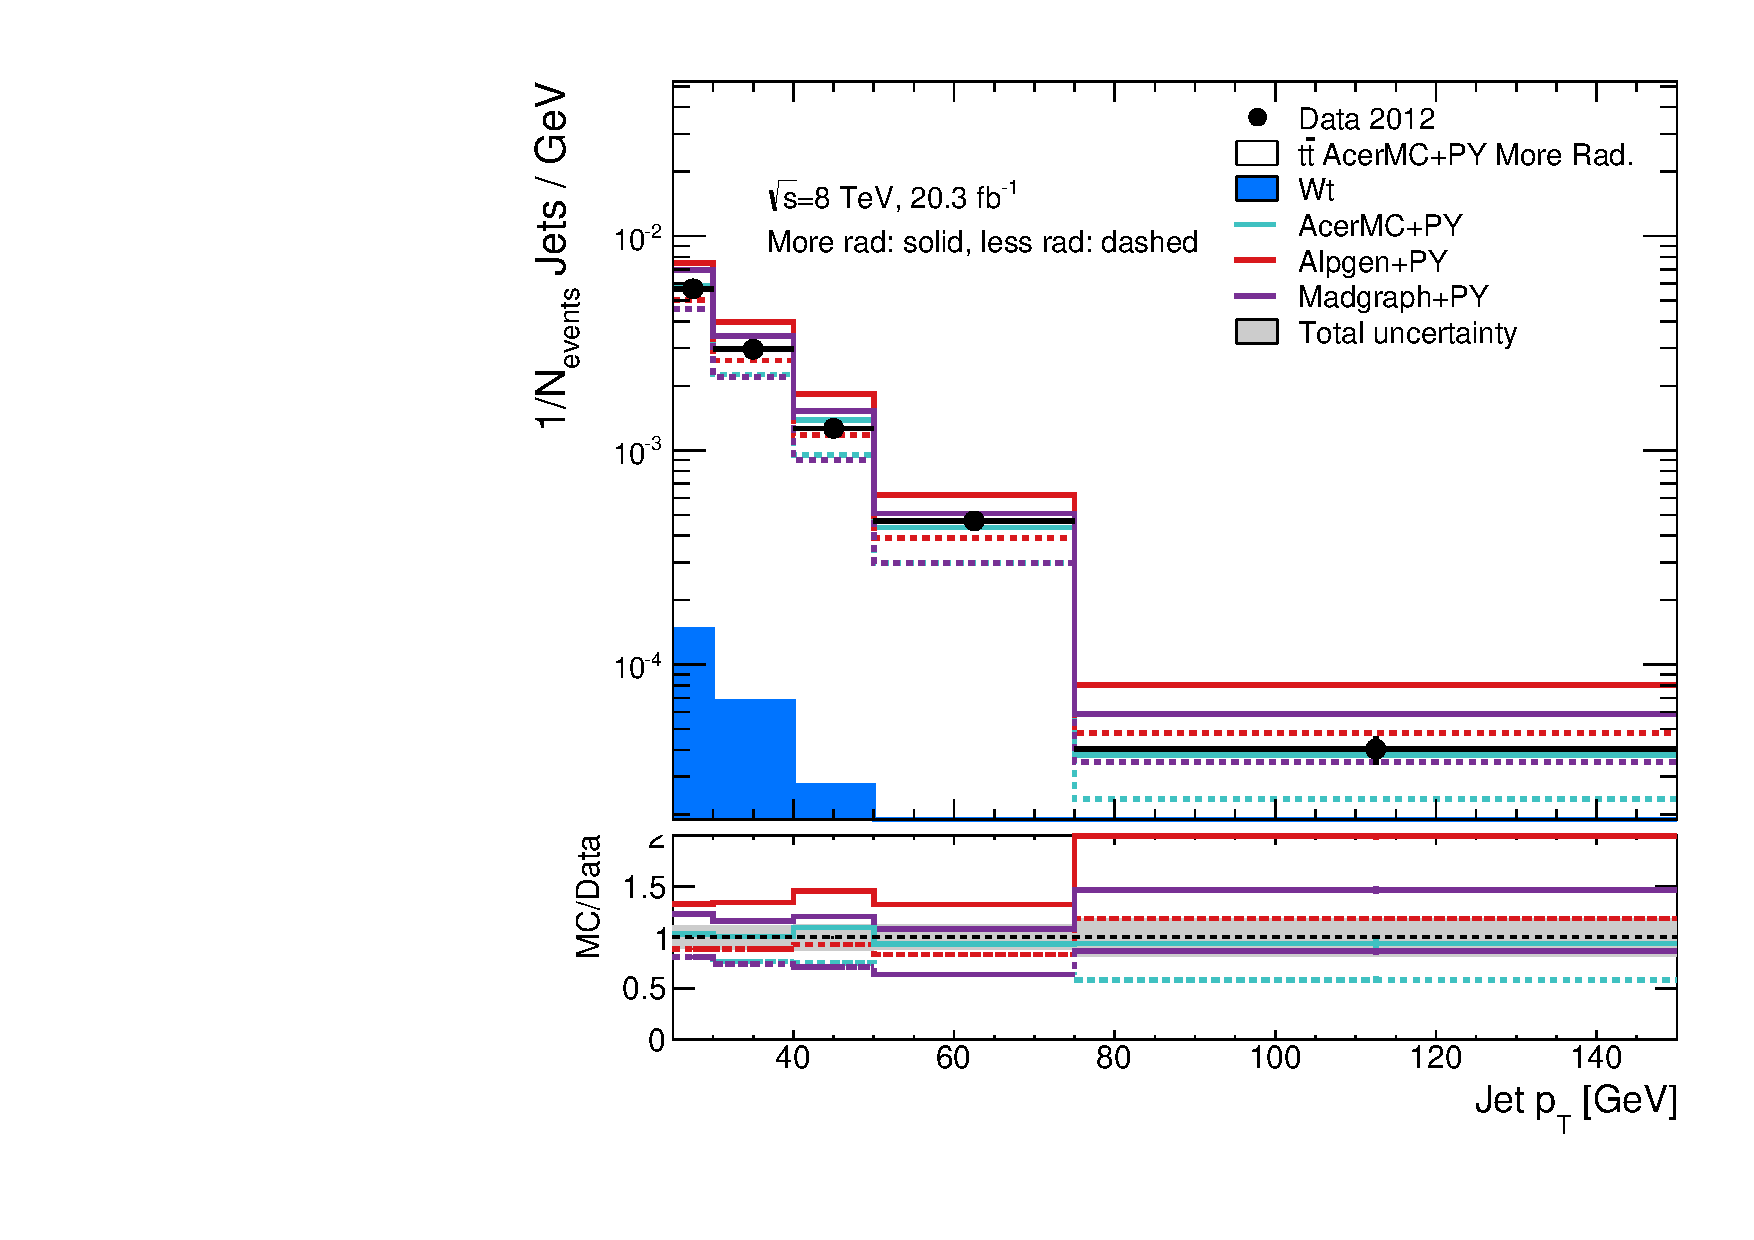
\includegraphics[width=0.45\textwidth]{fig/DataUnfold/LOSys/PtJet2.pdf}}
\subfloat{
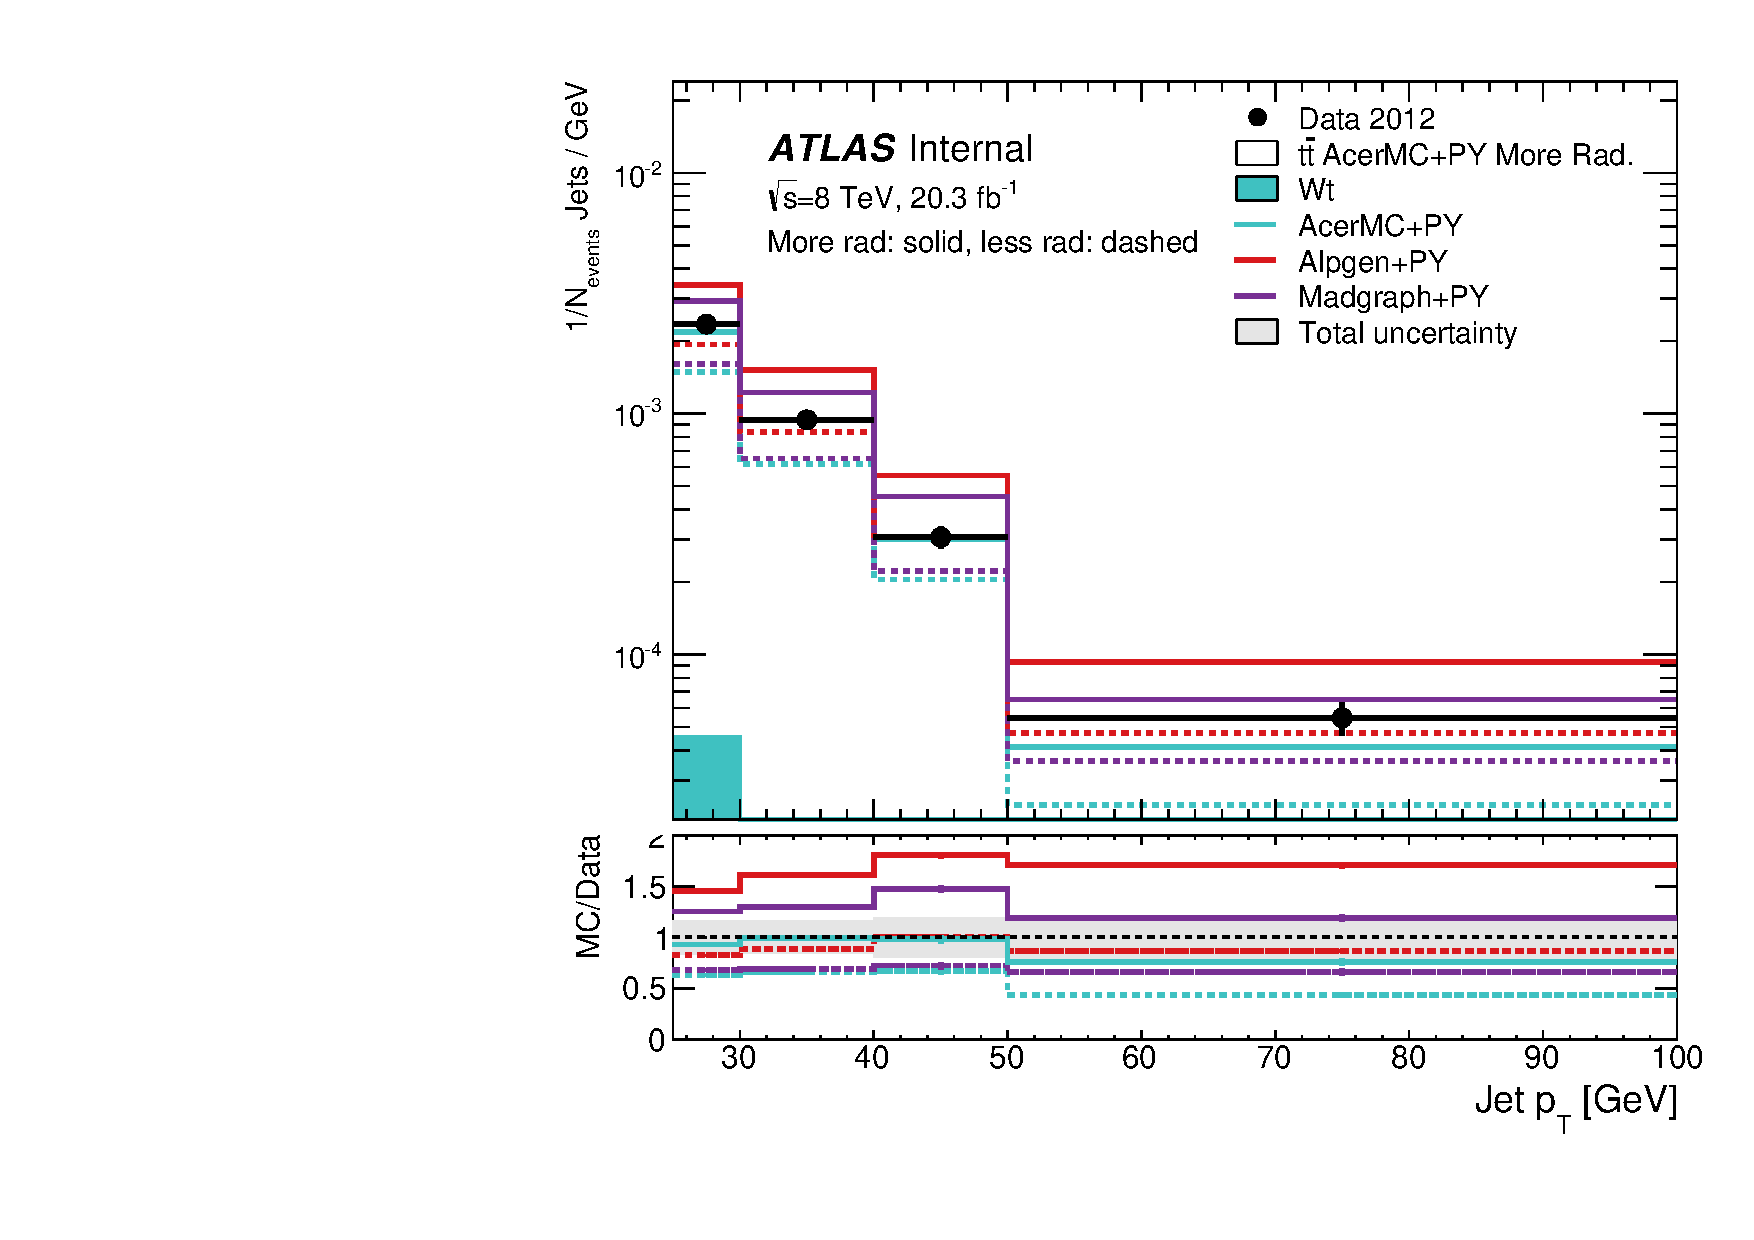
\includegraphics[width=0.45\textwidth]{fig/DataUnfold/LOSys/PtJet3.pdf}}%s \\
% \subfloat{
% 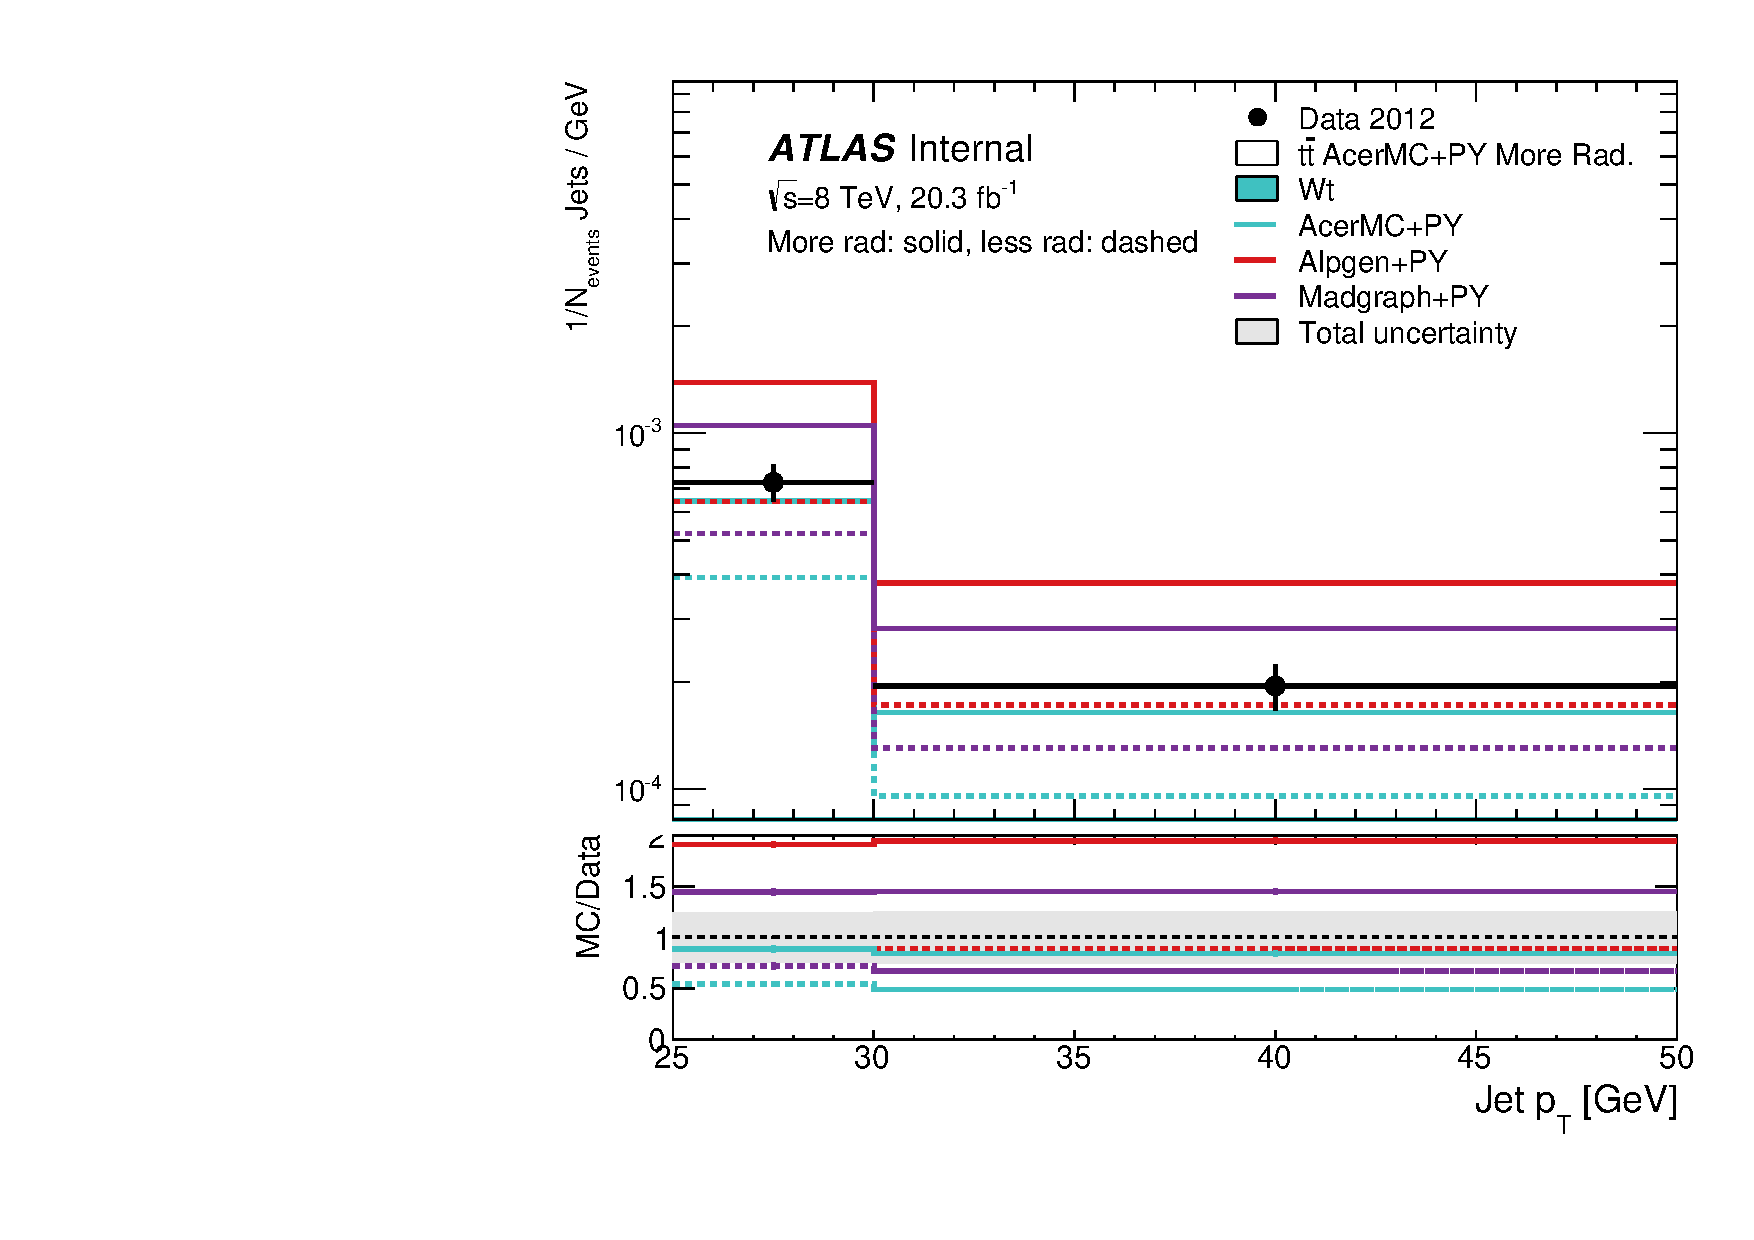
\includegraphics[width=0.45\textwidth]{fig/DataUnfold/LOSys/PtJet4.pdf}}
\caption{Distributions of the unfolded \pt of extra jets in data and simulation. Each sample is unfolded against a response matrix filled with baseline \ttbar+single top simulation. The gray band on the ratio shows the sum of statistical and systematic uncertainties.}
 \label{fig:unfptlosys}
 \end{figure}
 \section{\chisq\ comparisons and discussion}

Because the systematic and unfolding uncertainties have large correlations between bins,  
calculating the \chisq\ from the full covariance matrix is necesarry to assess the  agreement between the data and generators. Table~\ref{t:chi2} presents the $\chi^2$ obtained by comparing the  extra jet \pt\ and rank distributions in the data and each generator. The $\chi^2$ is calculated using only the statistical uncertainty, as well as the sum of systematic and statistcal uncertainties. The structure of \chisq\ can be be visualized as a matrix of its addends $(N^{i}_{mc}-N^{i}_{data})\sigma^{-1}_{ij}(N^{j}_{mc}-N^{j}_{data})^{j}$. This matrix is shown for \powpy, \hdamp, \madpy, and \peight\ in Figure~\ref{fig:chi2}.

Among NLO generators, \hdamp\ and \powpy\ agree the best with the data. \pow+\hw\ and \peight\ are slightly disfavored, and \mcnlohw\ is excluded. For multi-leg LO generators, \alpg+\py\ agrees well with data, while \madpy\ and \alpg+\hw\ are slightly disfavored. The less radiation systematic variation of \madpy\  agree best with data, suggesting that the scale used in baseline ATLAS tunes may predict too much radiation in this analysis' fidicual region. \acermc+\py\ does not reproduce the data well, regardless of scale.




\begin{table}
\begin{center}
\begin{tabular}{|l|cc|cc|}
\hline
Generator & $\chi^2_{\textrm stat}$ & $p$-value & $\chi^2_{\textrm{stat+sys}}$ & $p$-value \\
\hline
\powpy & 103.06 & 2.9628\e{-7} & 53.59 & 8.9931\e{-2} \\
\hdamp & 129.84 & 3.6708\e{-11} & 43.77 & 3.5480\e{-1} \\ 
\peight & 162.67 & 2.0444\e{-16} & 61.72 & 1.9762\e{-2} \\ 
\mcnlohw & 301.51 & 2.1411\e{-41} & 103.58 & 2.5140\e{-7} \\ 
\pow+\hw & 246.22 & 4.3310\e{-31} & 55.95 & 5.9838\e{-2} \\ 
%\powpy FS & 104.79 & 1.7104\e{-7} & 63.52 & 1.3584\e{-2} \\ 
\hline
\alpg+\hw & 162.34 & 2.3213\e{-16} & 74.80 & 9.8529\e{-4} \\ 
\alpg+\py & 147.24 & 6.7828\e{-14} & 50.71 & 1.4222\e{-1} \\
\madpy & 167.50 & 3.2078\e{-17} & 53.01 & 9.9021\e{-2} \\ 
\hline
\acermc+\py RadHi & 185.62 & 2.6851\e{-20} & 116.39 & 3.8078\e{-9} \\  
\acermc+\py RadLo & 401.24 & 1.2019\e{-60} & 95.75 & 2.8533\e{-6} \\  
\alpg+\py RadHi  & 709.83 & 7.6068\e{-123} & 104.70 & 1.7642\e{-7} \\  
\alpg+\py RadLo  & 124.23 & 2.6195\e{-10} & 45.51 & 2.8983\e{-1} \\ 
\madpy $q^{2}$ down  & 187.13 & 1.4771\e{-20} & 55.47 & 6.5133\e{-2} \\  
\madpy $q^{2}$ up  & 506.35 & 1.6412\e{-81} & 95.84 & 2.7788\e{-6} \\ 
\hline

\end{tabular}
\caption{$\chi^2$ between extra jet \pt\ spectra in fully corrected data and different generators. The first column represents the agreement including only (diagonal) statistical uncertainties. The second column also includes the covariance due to systematic uncertainties (primarily JES).} 
\label{t:chi2}
\end{center}
\end{table}

\begin{figure}
\centering
\subfloat{
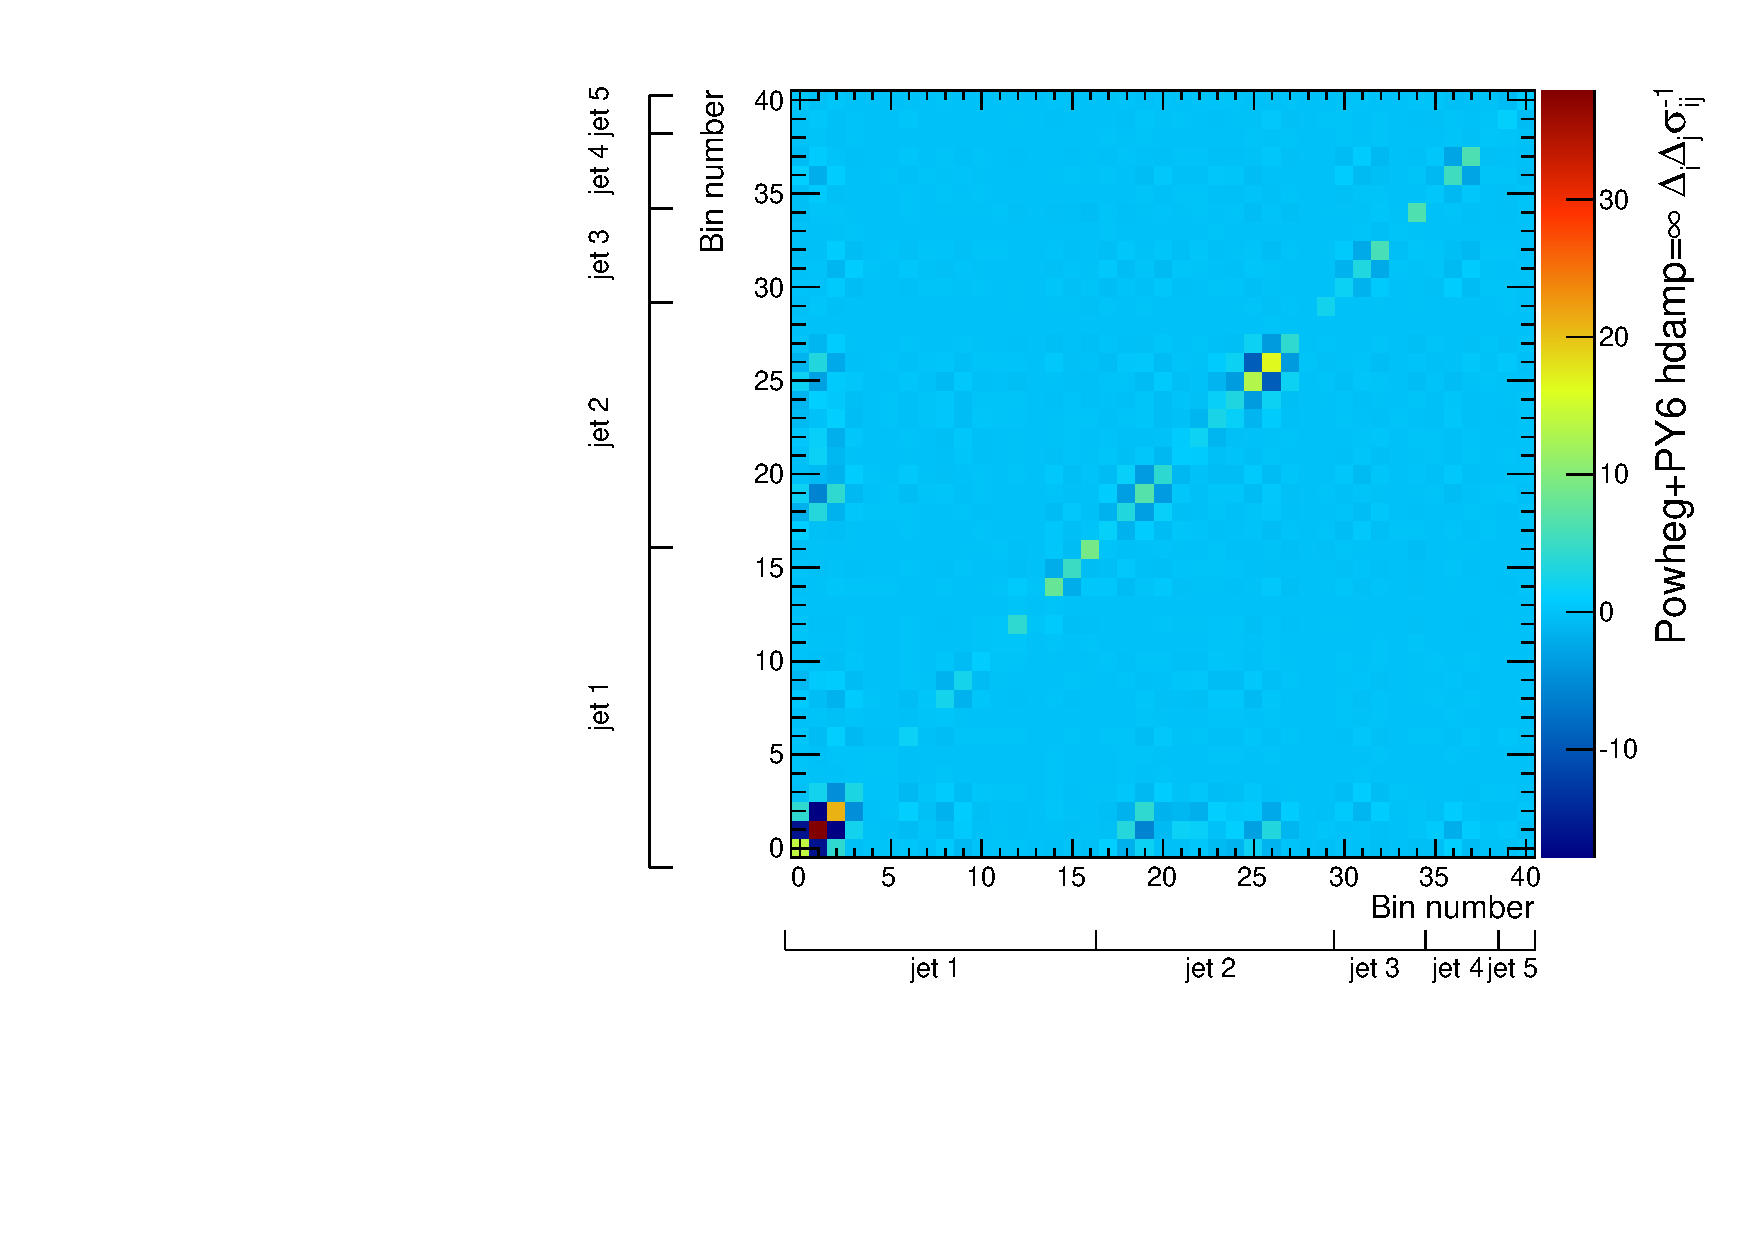
\includegraphics[width=0.45\textwidth]{fig/DataUnfold/NLOFS/Chi2/117050atlfast.pdf}
} 
~
\subfloat{
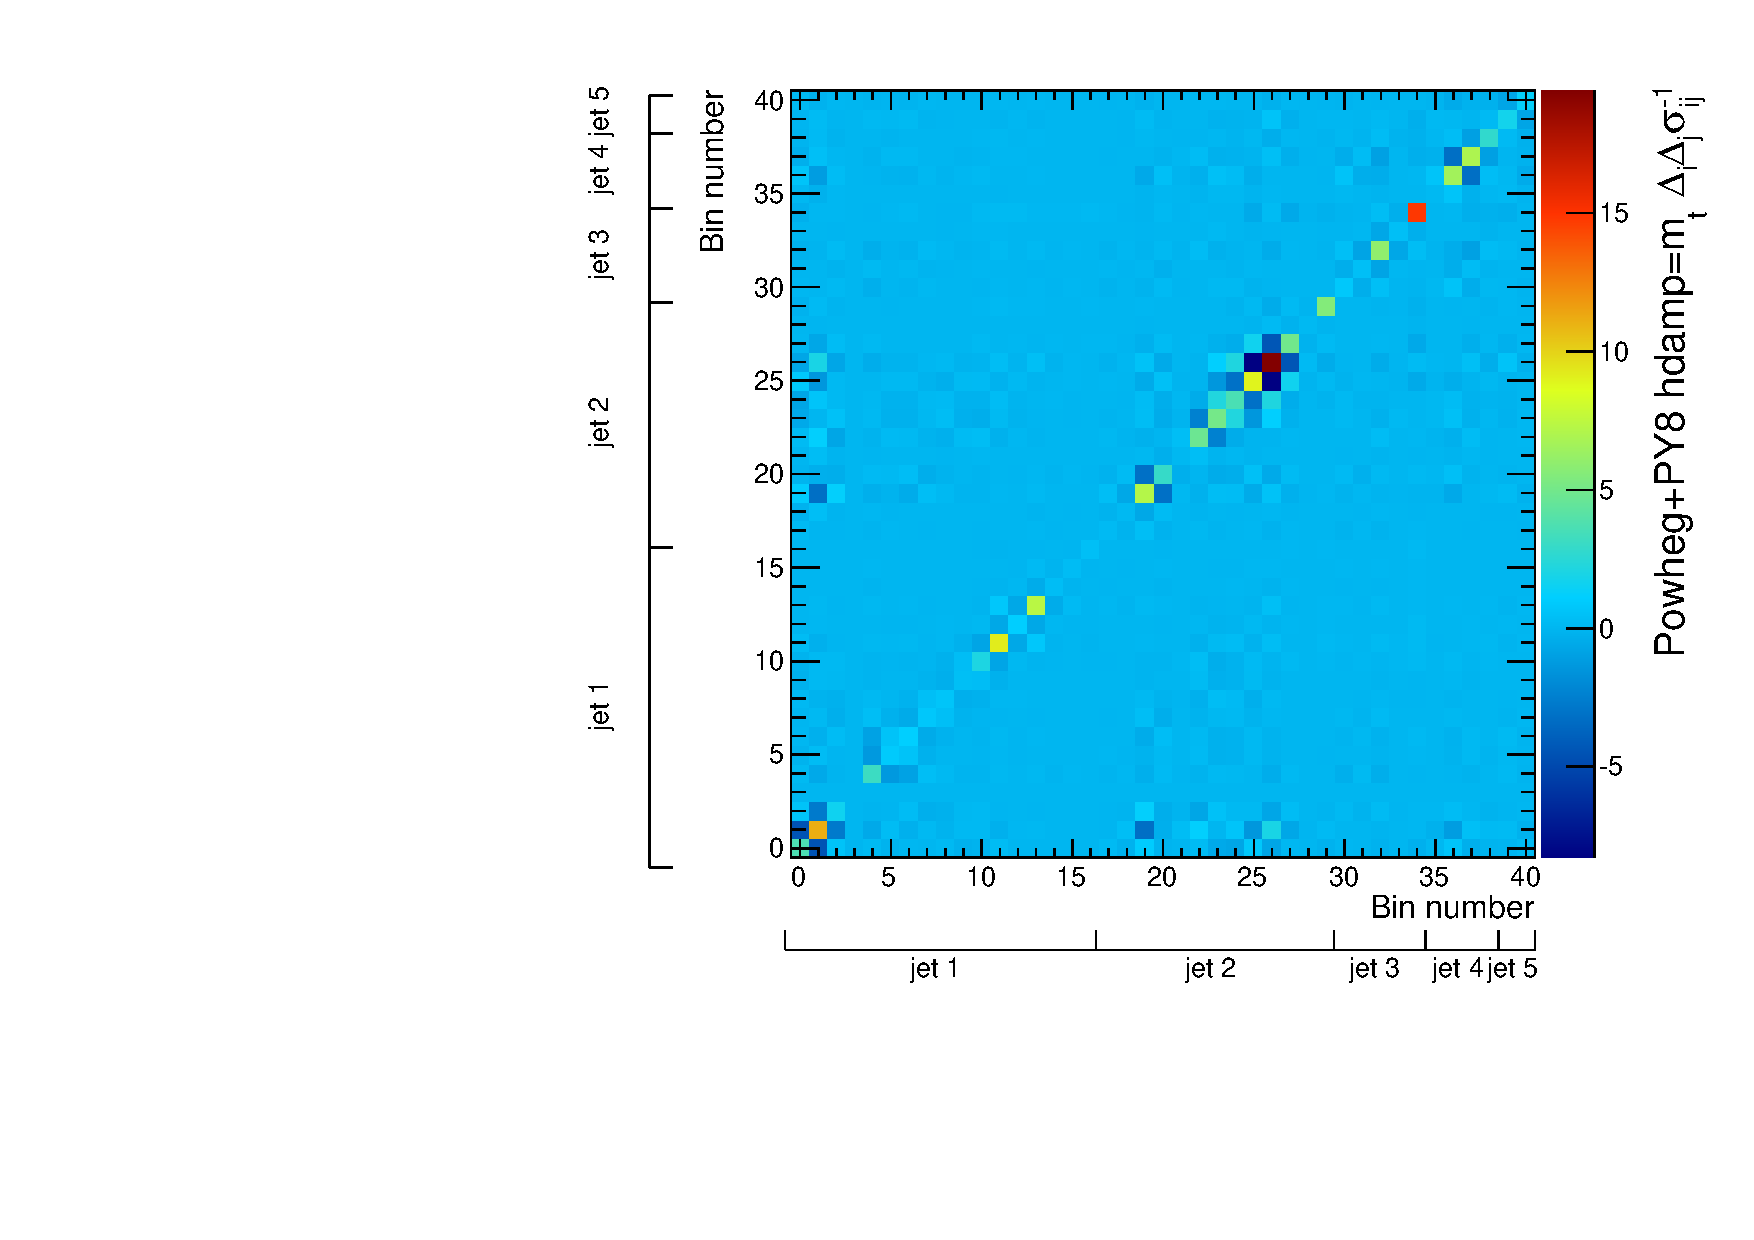
\includegraphics[width=0.45\textwidth]{fig/DataUnfold/NLOFS/Chi2/117046atlfast.pdf}}
\\
\subfloat{
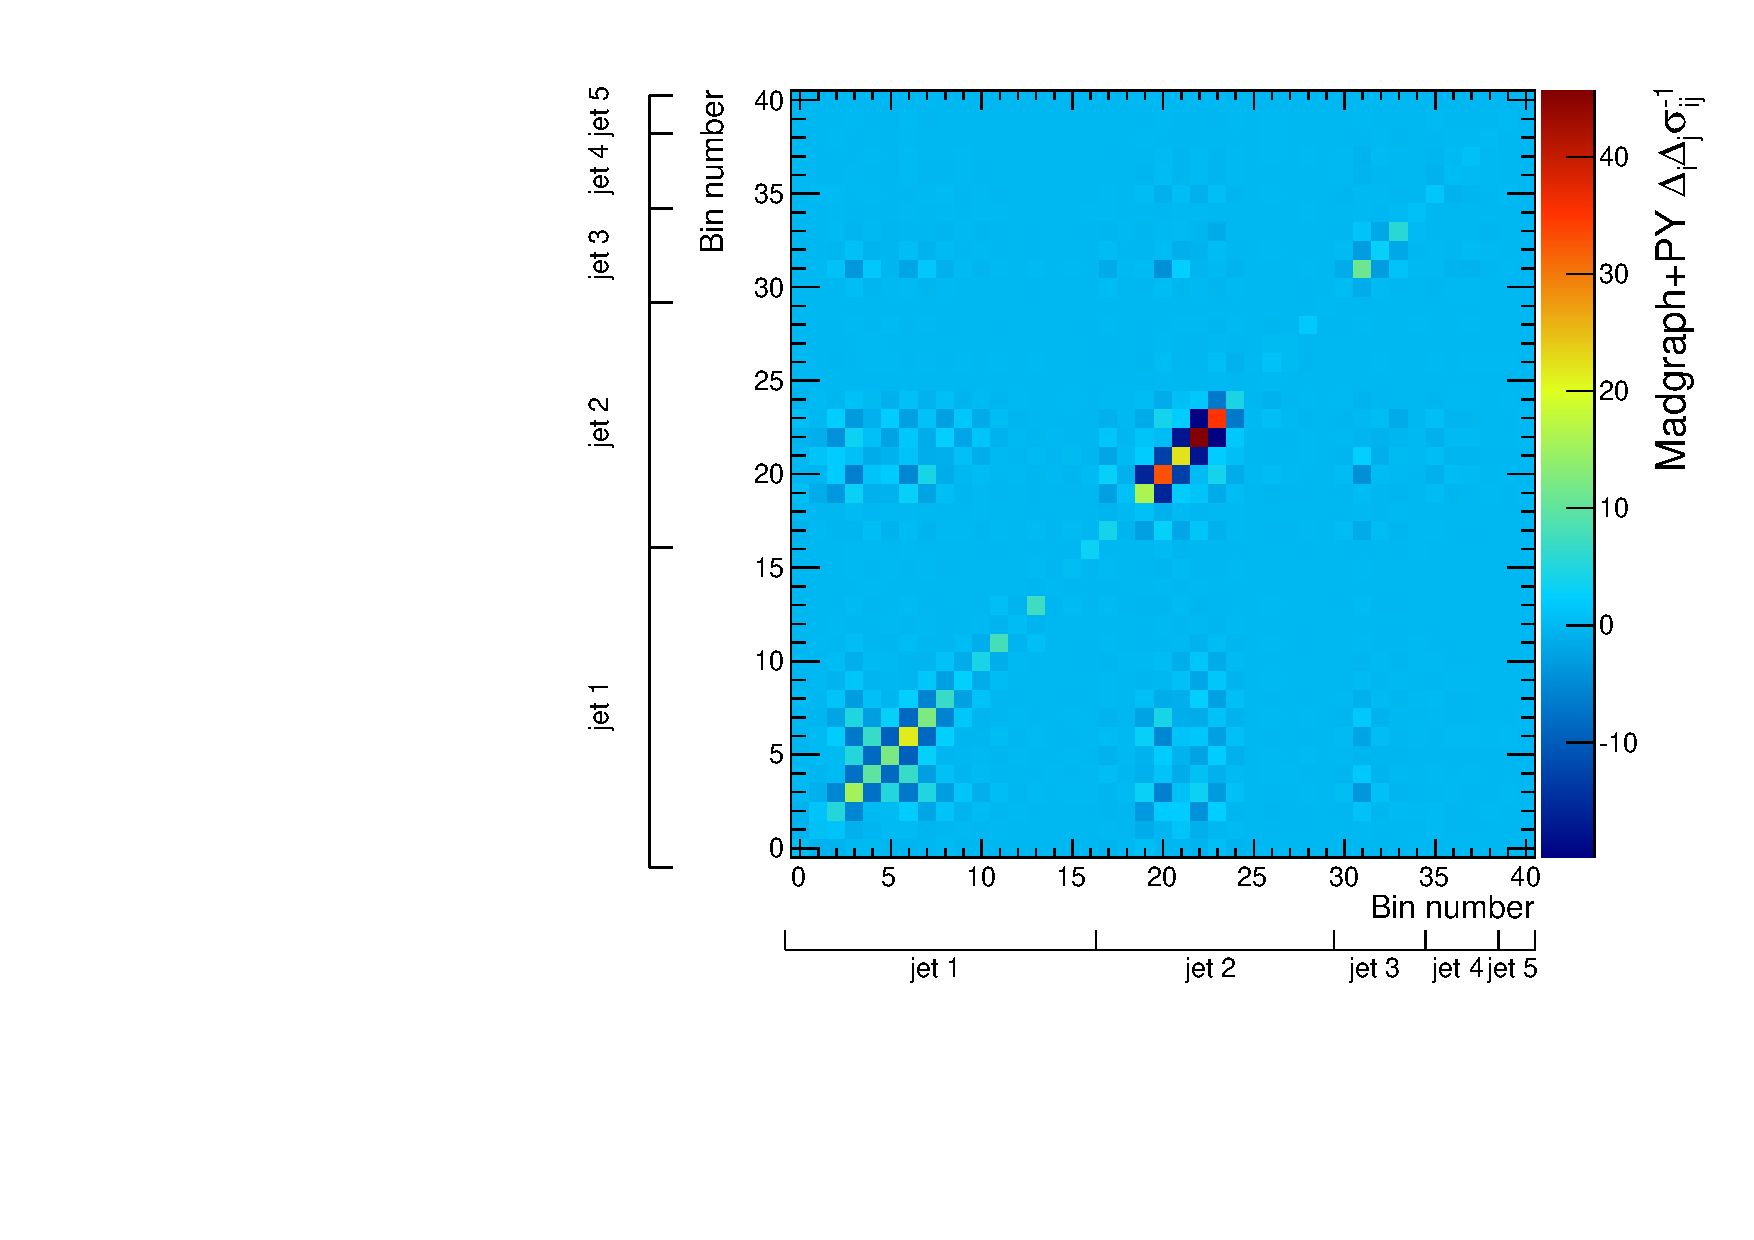
\includegraphics[width=0.45\textwidth]{fig/DataUnfold/LOMultiLeg/Chi2/110872atlfast.pdf}}
~
\subfloat{
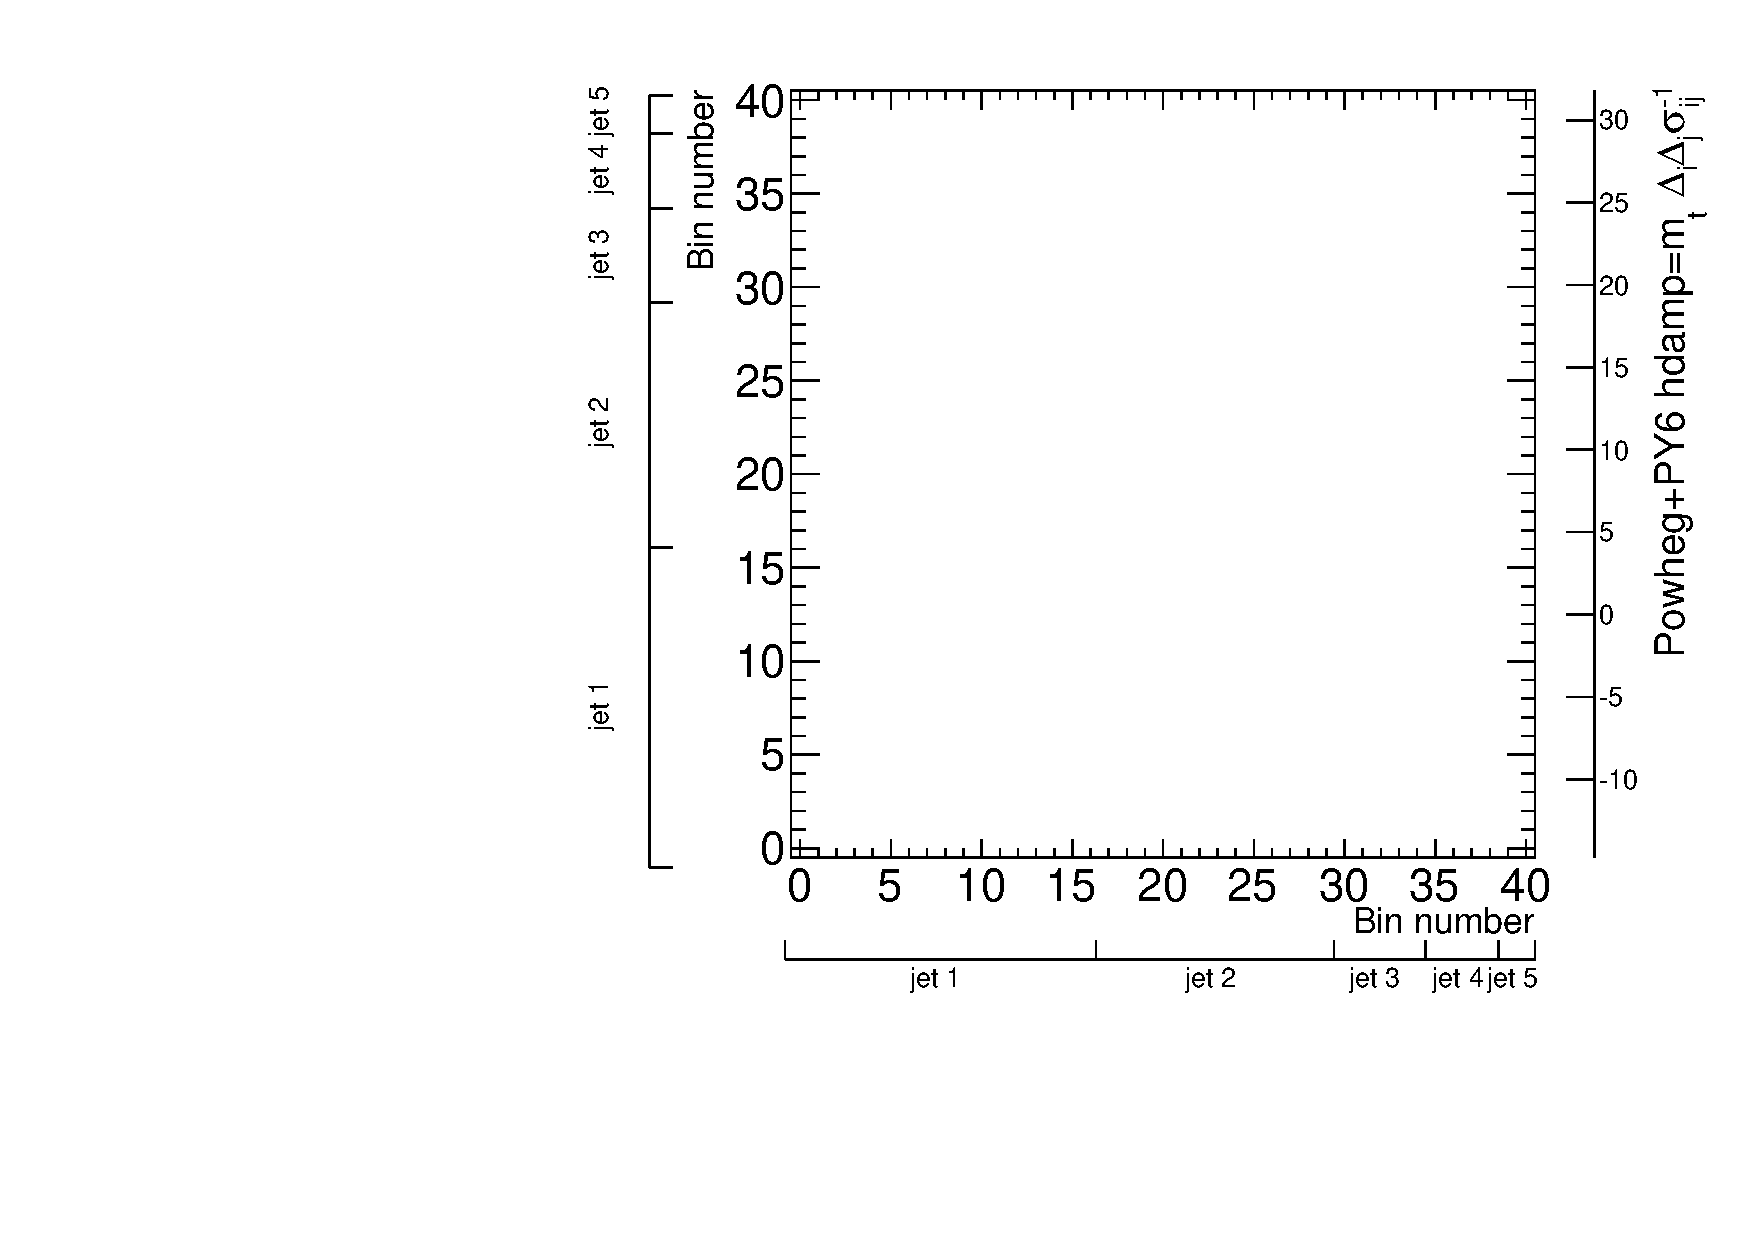
\includegraphics[width=0.45\textwidth]{fig/DataUnfold/NLOFS/Chi2/110404atlfast.pdf}}
~
\caption{Visual representation of the $\chi^2$ distributions for (a) \powpy\ (b) \peight\ (c)  \madgraph +\py\  and (d) \hdamp. Each element $ij$ of the matrix is given by $M_{ij}=(N^{i}_{mc}-N^{i}_{data})\sigma^{-1}_{ij}(N^{j}_{mc}-N^{j}_{data})^{j}$ where $N^{i}_{mc}$ is the number of jets predicted in bin i, $N^{i}_{data}$ is the number of jets in bin $i$ in data, and $\sigma^{-1}$ is the inverse of the covariance matrix.}
\label{fig:chi2}
\end{figure}

